\section{Unternehmen}
Die allink GmbH wurde 2005 von den drei Partner David Zangger, Christoph Schlatter
und Michael Walder gegründet. David Zangger und Christoph Schlatter kümmern sich
seit jeher als Creative Directors um die grafischen Umsetzungen und die Designqualität.
Michael Walder kümmerte sich bis 2010 nebst den geschäftsführerischen Tätigkeiten
auch um die ganze Informatik. Nach der Fusionierung mit der SiSprocom übergab
er die Leitung der Informatik an mich ab und widmet sich nun dem Aufbau der
Beratung und Projektleitung. Seit 2010 bezeichnet wir uns als die interdisziplinäre 
und marktnahe Designagentur.

\begin{quote}
allink.creative ist eine Designagentur, die Produkte, Marken und Unternehmen 
attraktiv und einzigartig in Szene setzt. Unser Design soll Menschen erreichen 
und begeistern. Weil wir marktnah arbeiten, stellen wir den wirtschaftlichen 
Nutzen von Design stets in den Vordergrund.

Wir arbeiten interdisziplinär, damit wir die breiten Möglichkeiten an 
Kommunikationskanälen optimal für unsere Kunden einsetzen können. Unser 
Team von Spezialisten aus den vielfältigsten Bereichen findet innovative 
und gesamtheitliche Lösungen, um Marken und Firmen wirkungsvoll zu positionieren. 
Die Bereiche Branding, Online Communication, Packaging Design und Product 
Design zählen dabei zu unseren Kernkompetenzen.
\end{quote}

Das Unternehmen lässt sich zur Zeit in die drei Hauptbereiche Beratung, Grafik
und Informatik unterteilen. In einer funktionalen Struktur sieht das bei allink wie in
der Grafik \ref{pic:funktionales_organigramm} abgebildet aus.

\begin{figure}[htbp]
\begin{center}
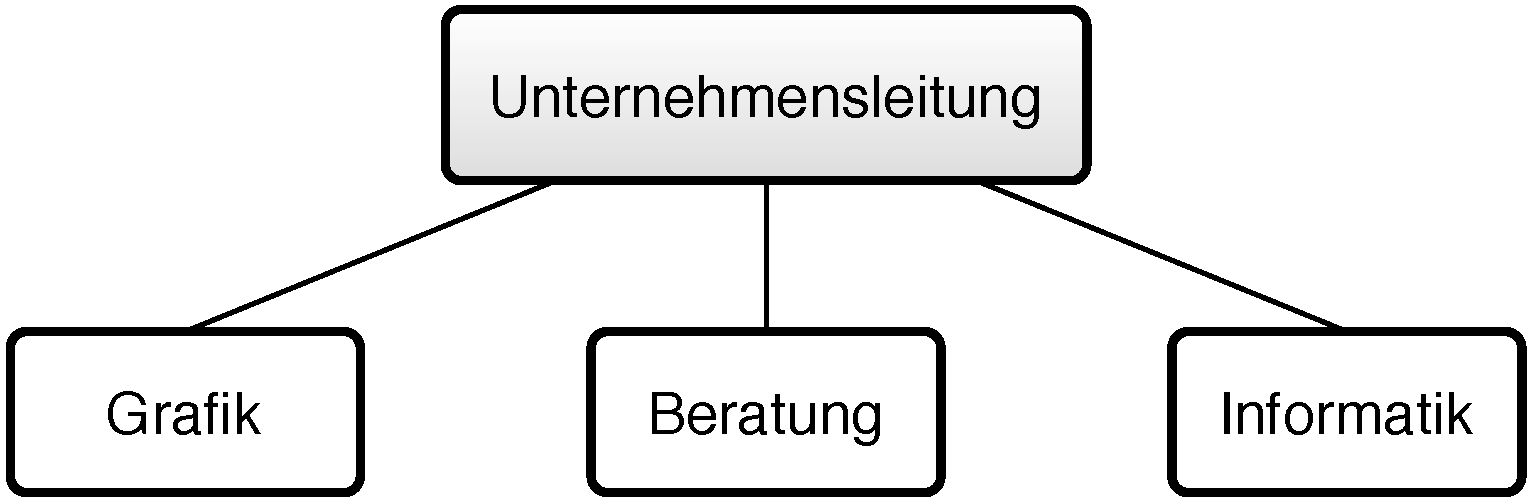
\includegraphics[width=0.45\textwidth,angle=0]{./bilder/funktionales_organigramm.pdf}
\caption{Funktionales Organigramm von allink}
\label{pic:funktionales_organigramm}
\end{center}
\end{figure}

Wobei sich jeweils ein bis zwei Partner um einen
Bereich kümmern. Dies beinhaltet nebst den Alltagsarbeiten auch organisatorische 
Aufgaben wie das Einstellen von neuen Mitarbeitern, die Verteilung der Arbeiten an den 
passendsten Mitarbeiter in dessen Bereich und natürlich auch Entlassungen.
In der Grafik \ref{pic:mitarbeiter_pro_bereich} sind die Mitarbeiter pro Bereich
abgebildet.

\begin{figure}[htbp]
\begin{center}
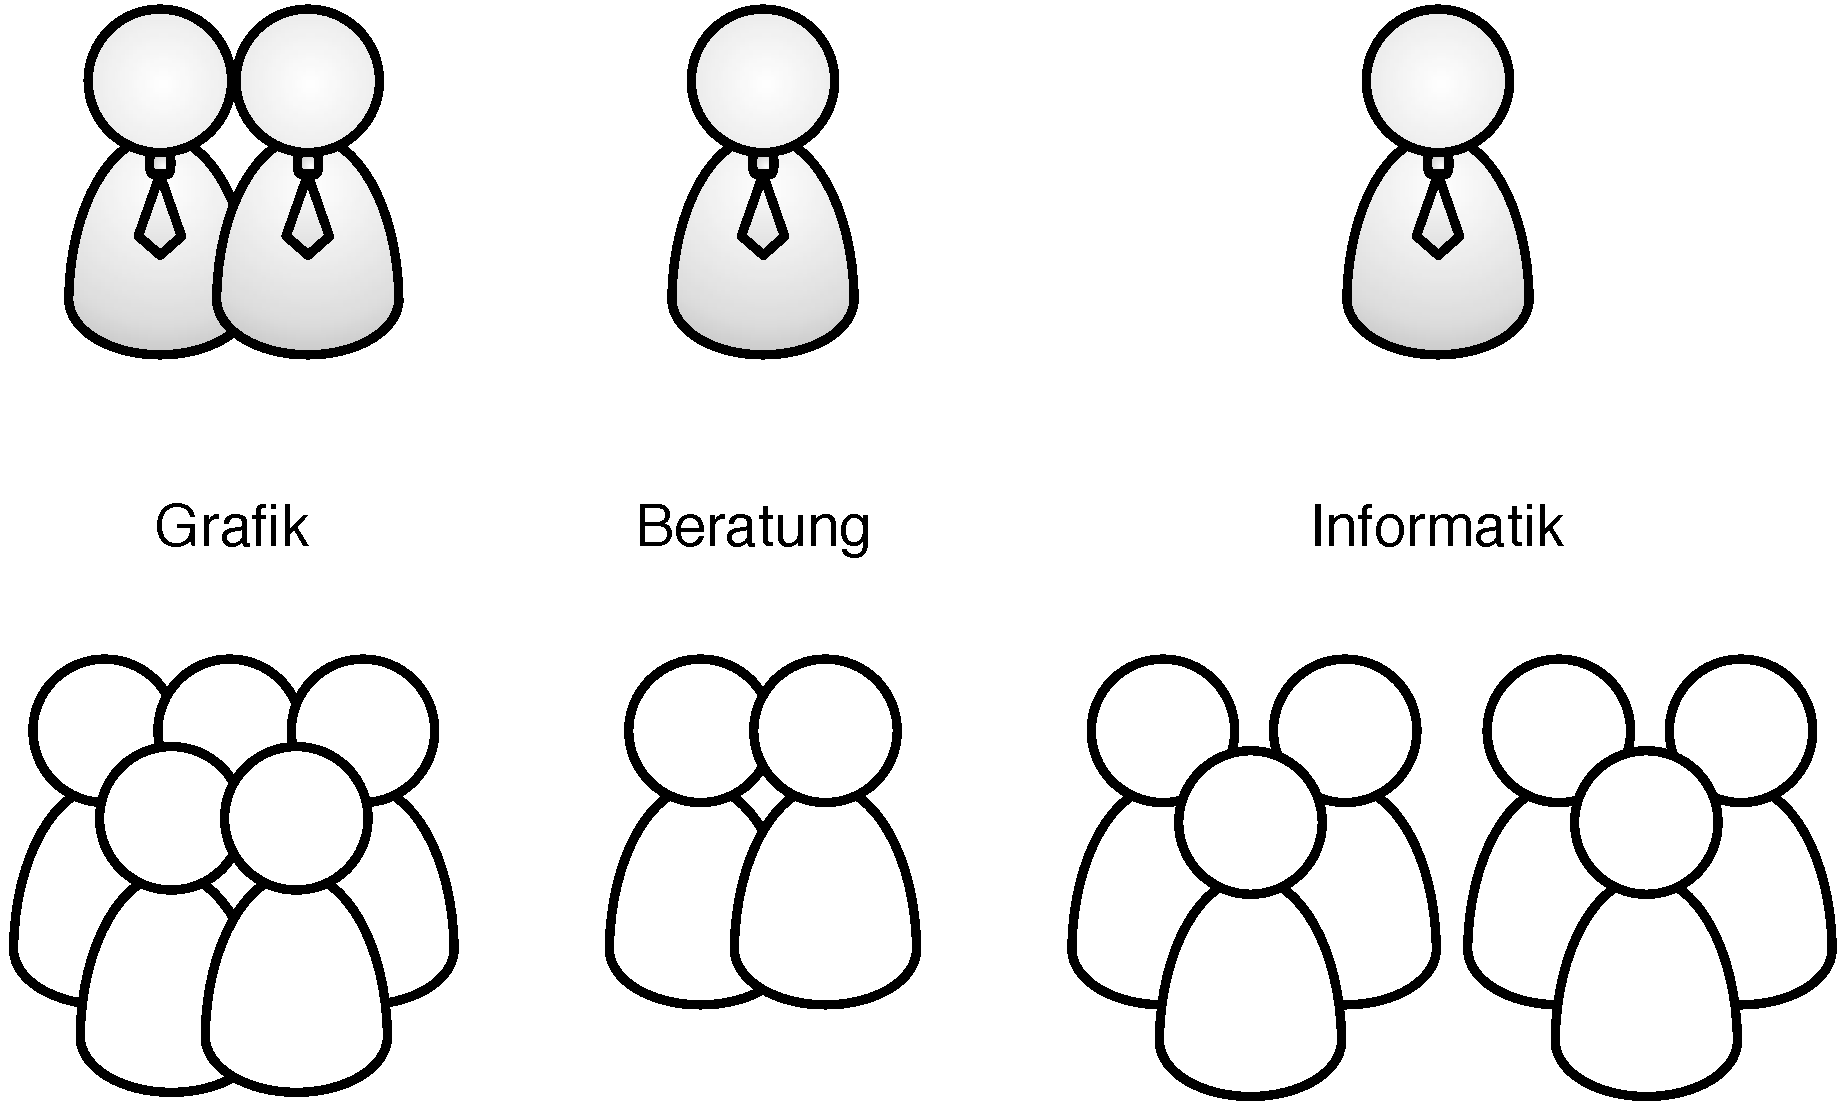
\includegraphics[width=0.55\textwidth,angle=0]{./bilder/mitarbeiter_pro_bereich.pdf}
\caption{Übersicht der Mitarbeitern pro Bereich}
\label{pic:mitarbeiter_pro_bereich}
\end{center}
\end{figure}

In der Grafik sind nebst drei Vollzeitangestellen noch ein Praktikant und eine
Lehrtochter angestellt. In der Beratung beschäftigen wir zur Zeit zwei Mitarbeiter.
Und die Informatik setzt sich aus zwei Vollzeitangestellten sowie einem Pratikant
zusammen. Die drei weiteren Informatiker arbeiten als externe Consultants und
werden höchst selten in einem internen Projekt beschäftigt.

Trotz dieser Aufteilung in mehrere Bereiche geht der Kommunikationsweg nicht
immer über die für den Mitarbeiter zuständigen Partner. 

\begin{figure}[htbp]
\begin{center}
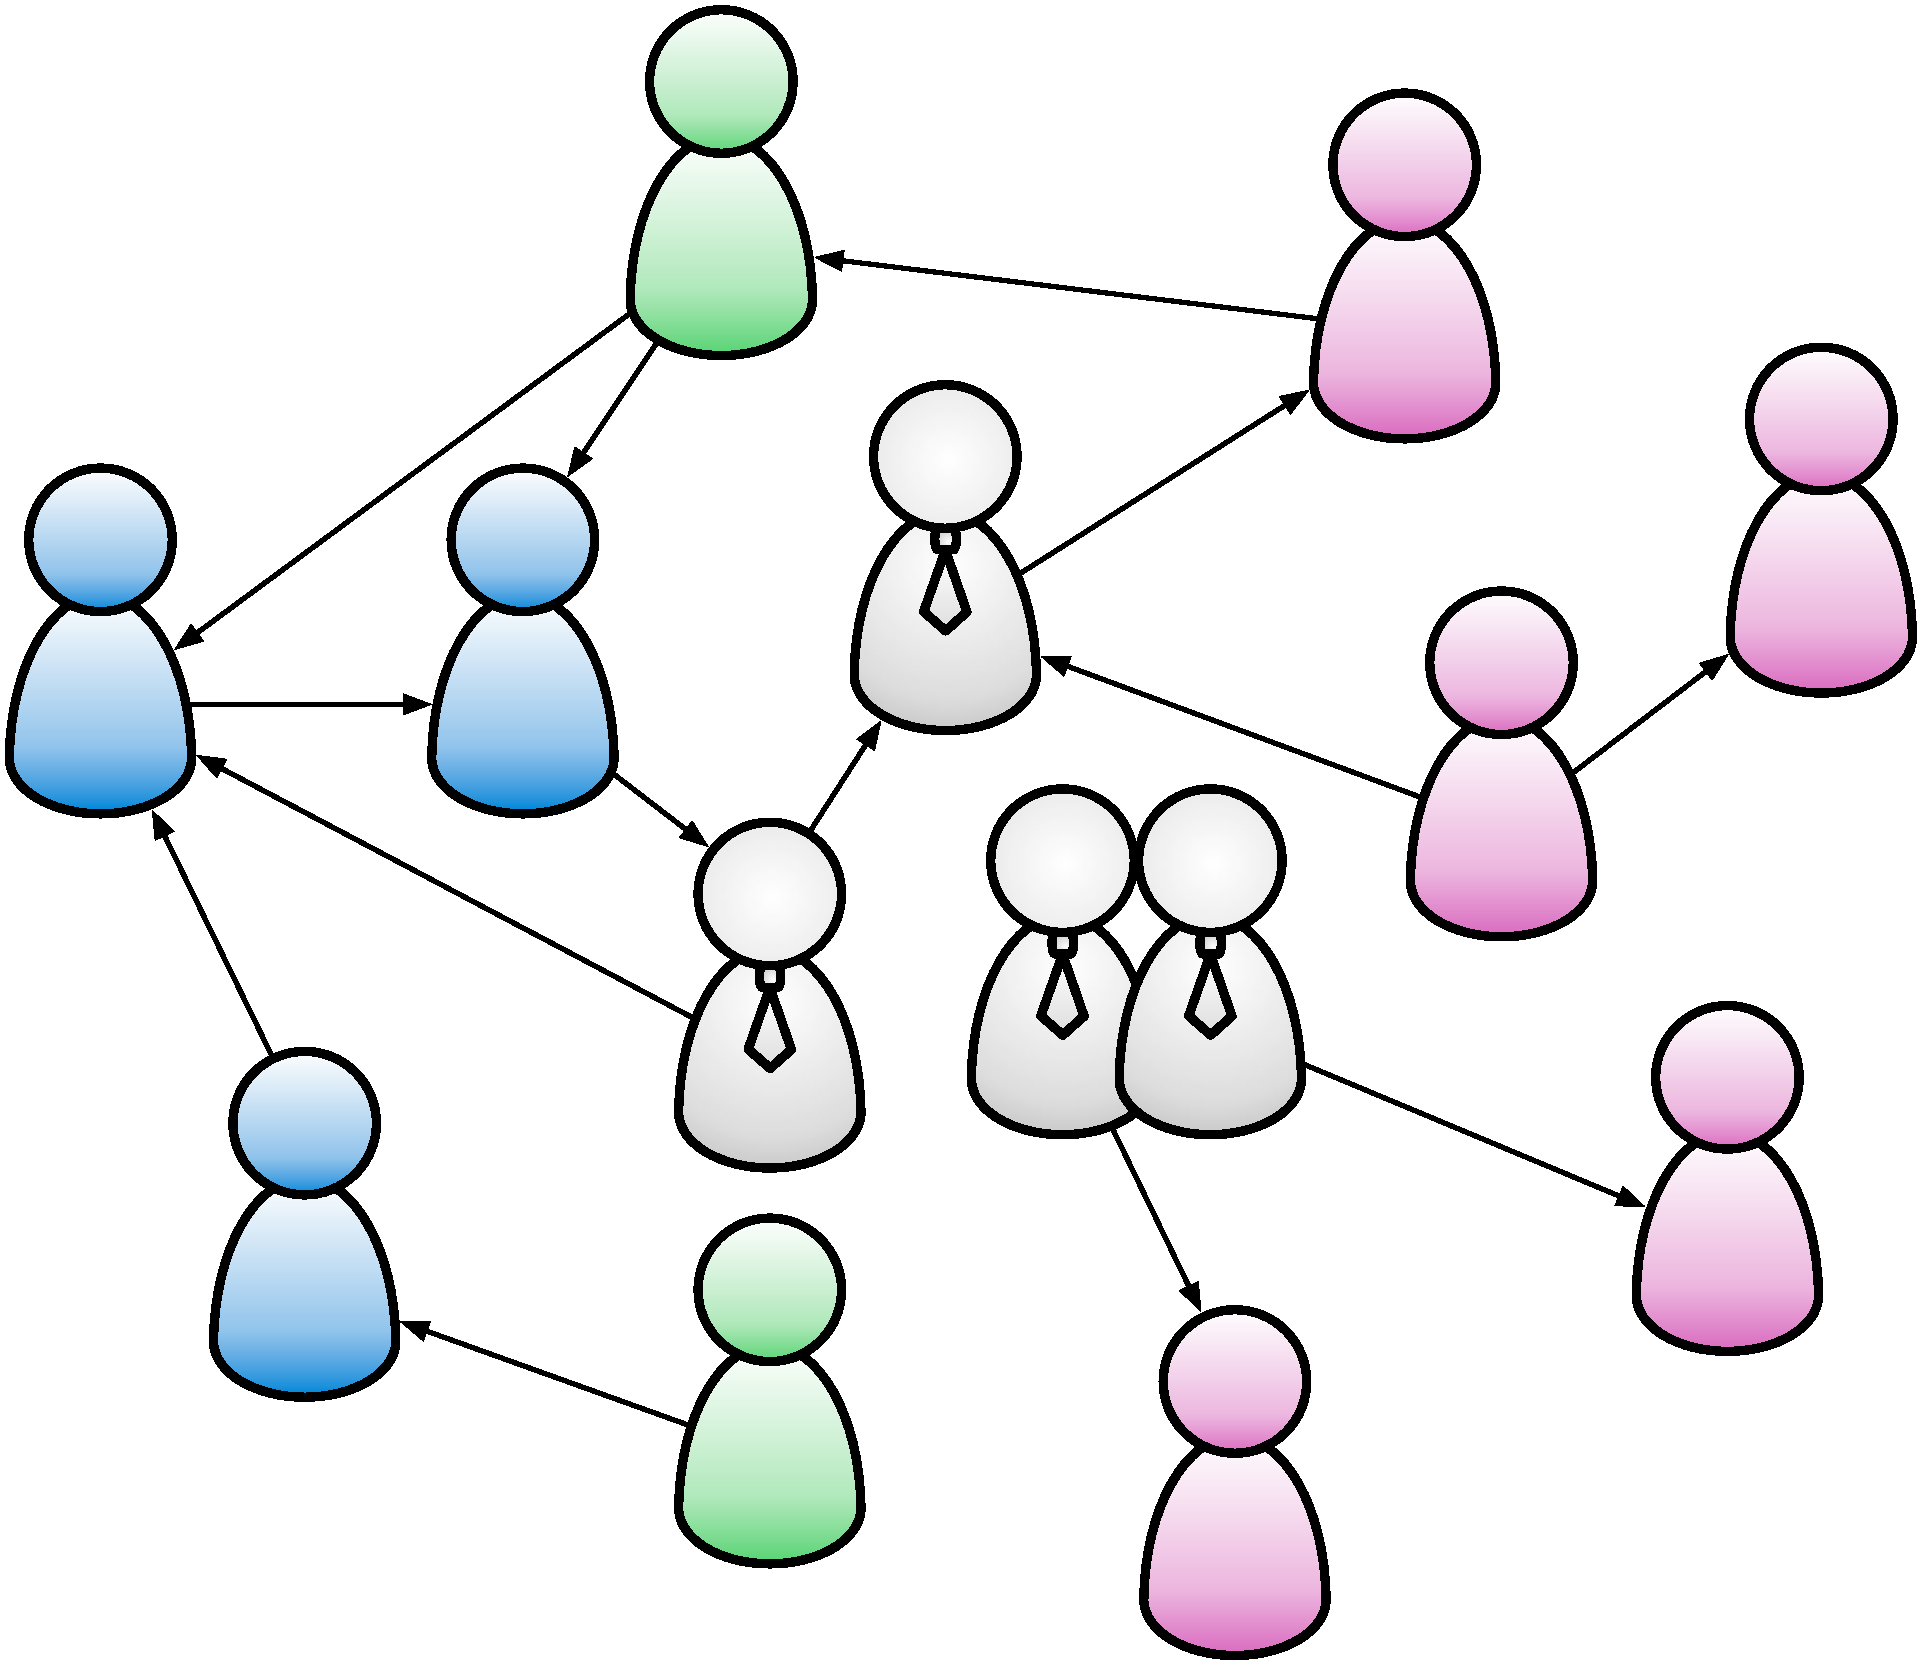
\includegraphics[width=0.40\textwidth,angle=0]{./bilder/kommunikationswege.pdf}
\caption{Beispiel der unorganisierten Kommunikationswege}
\label{pic:kommunikationswege}
\end{center}
\end{figure}

Das ist auch grundsätzlich nicht zu vermeiden, bzw. das muss zu einem gewissen
Grad auch der Fall sein. Ansonsten wären die Abläufe von wenigen Anlaufstellen abhängig
und das ganze würde ins Stocken geraten. Trotzdem birgt es gewisse Schwachstellen.
Zum Beispiel, dass nicht alle Beteiligten eines Projektes den gleichen Informationstand 
haben. Dies kann sich beim Kontakt mit einem Kunden negativ auswirken, wenn der
Kunde zum Beispiel schon über etwas informiert wurde, und der Mitarbeiter am
Telefon selbst gar noch nicht weiss. Die Schwächen beleuchte ich in der Analyse
des Projektablaufes noch genauer.

Der Aufbau einer Beratung, die zur Zeit im Gange ist, soll genau solche Probleme
lösen. Jedoch stecken wir hier noch in den Kinderschuhen und erhoffen uns aus
dieser Arbeit Erkenntnisse über einen möglichst optimalen Projektablauf.

\section{Kunden}
Im Gegensatz zur SiSprocom hat die allink einen relativ grossen Kundenstamm.
Das bedeutet, dass kein grosses Klumpenrisiko existiert. Jedoch ist auch
die Auftragskontinuität der einzelnen Kunden viel kleiner. Für manche arbeiten
wir jeden Monat an einem neuen Projekt, für anderen einmal im Jahr.
In der Grafik \ref{pic:kundenauszug} ist ein Teil unserer Kunden abgebildet.

\begin{figure}[htbp]
\begin{center}

\includegraphics[width=0.8\textwidth,angle=0]{./bilder/kundenauszug.jpg}
\caption{Kundenauszug von allink}
\label{pic:kundenauszug}
\end{center}
\end{figure}

Unterteile ich unsere Kunden in die gängigen Firmengrössen Kleinstunternehmen,
kleine Unternehmen und mittlere Unternehmen, so gelange ich zu einer interessanten 
Verteilung. Die Definition der Unternehmensgrössen basiert auf einer Empfehlung
der Kommission der Europäischen Union\footnote{\citealp*[Vgl.][Anhang Art. 2]{eu_komission_unternehmen}}.
Diese unterteilt die Unternehmen nach dem in der 
Tabelle \ref{tab:eu_unterteilung} abgebildetem Schlüssel.

\begin{table}[h]
\begin{center}
    \begin{tabular}{clccccc}
        \toprule \textbf{Typ} & \textbf{Beschäftigte} & & \textbf{Umsatzerlös} & & \textbf{Bilanzsumme} \\
        \midrule Kleinstunternehmen & $<$ 10 & und & $\leq$ 2 Mio \euro & oder & $\leq$ 2 Mio \euro \\
        \midrule Kleine Unternehmen & $<$ 50 & und & $\leq$ 10 Mio \euro & oder & $\leq$ 10 Mio \euro \\
        \midrule Mittlere Unternehmen & $<$ 250 & und & $\leq$ 50 Mio \euro & oder & $\leq$ 43 Mio \euro \\
        \bottomrule
    \end{tabular}
    \caption{Empfehlung Unternehmensunterteilung, Kommission der Europäischen Union}
    \label{tab:eu_unterteilung}
\end{center}
\end{table}

Meine Kategorisierung unserer Kunden, abgebildet in der nachstehenden Grafik \ref{pic:kundenkategorisierung},
basiert überwiegend auf den Informationen von moneyhouse\footnote{moneyhouse bietet Handelsregister- und Firmendaten, \url{http://www.moneyhouse.ch}}, 
da ich nicht alle Kunden um aktuelle Mitarbeiter- und Umsatzzahlen bitten wollte
und aus zeitlichen Gründen auch nicht konnte. Zusätzlich zu den in der Tabelle 
\ref{tab:eu_unterteilung} aufgelisteten Kategorien habe ich noch die Kategorie 
``Grosse Unternehmen'' hinzugefügt, um Firmen mit genau oder mehr als 250 
Mitarbeiter kategorisieren zu können.

Ich füge die vollständige Liste unserer Kunden und deren Kategorisierung absichtlich
nicht bei, da ich nicht alle Kunden in dieser Arbeit namentlich auflisten möchte.
Bei Bedarf kann die Liste aber bei uns eingesehen werden.

\begin{figure}[htbp]
\begin{center}
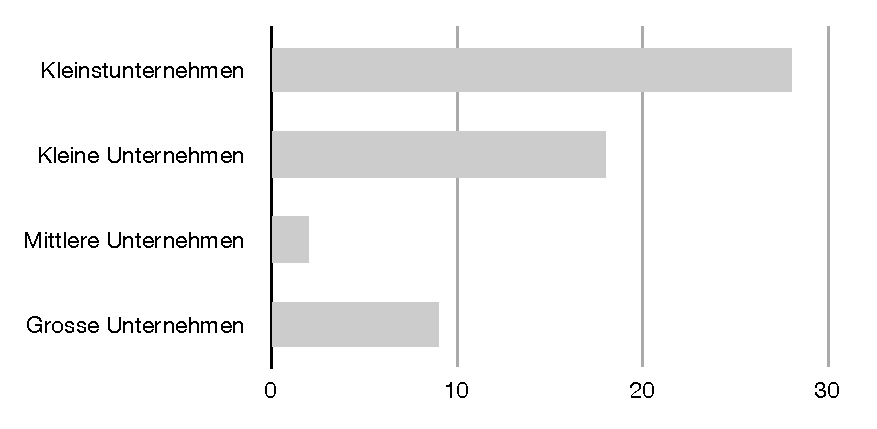
\includegraphics[width=0.75\textwidth,angle=0]{./bilder/analyse/kundenkategorisierung.pdf}
\caption{Anzahl Kunden der allink in Unternehmensgrössen kategorisiert}
\label{pic:kundenkategorisierung}
\end{center}
\end{figure}

Wie man erkennen kann, arbeiten wir überwiegend mit Kleinst- und kleinen 
Unternehmungen zusammen. Interessanterweise aber mehr grosse als mittlere
Unternehmen.
Die verschiedenen Firmenkulturen unserer Kunden haben natürlich auch einen Einfluss 
auf unsere Projektabläufe. Grundsätzlich stellen sich wohl alle Kunden
der Herausforderung, ihre Projekte gut zu organisieren. Je nach Auflagen oder
Abläufe der Kunden, hat dies auch Auswirkungen auf unseren Projektablauf.
Deshalb wäre es falsch anzunehmen, dass wir zur Zeit bei jedem Projekt und 
Kunden das selbe Vorgehen anwenden können.

Möglicherweise genau deshalb existiert zur Zeit kein definierter Projektablauf
bei allink. Doch gibt es klar erkennbare Gemeinsamkeiten in allen Projekten,
bzw. Projektabläufe. Ich werde im nächsten Kapitel \ref{chap:projektablauf} 
versuchen, den heutigen Projektablauf so abzubilden, dass er für die meisten
vergangenen Projekte Gültigkeit hat.

\section{Projektablauf}\label{chap:projektablauf}
Den heutigen Projektablauf bei der allink könnte man am Besten als ``natürliches Vorgehen''
umschreiben. Ein potentielles Projekt kommt an einen Partner heran, entweder über 
eine Anfrage oder eine Akquisition, der spricht sich mit den anderen Partner ab 
und nimmt dann die Mitarbeiter mit in das Projekt, die er als nötig erachtet.
Dies kommt einem Projektmanamgement organisiert über die Linie am nächsten.

Der Projektablauf wird in drei Prozesse, die Projektannahme und Offertenerstellung,
die Projektdurchführung und der Projektabschluss unterteilt und dazu die 
Ablaufdiagramme erstellt. Darin wird jede Aktion mit einer eindeutigen Nummer versehen,
um danach darauf im beschreibenden Text verweisen zu können. Nach einer Entscheidung erhöht
sich die Laufnummer jeweils um eine ganze Zahl, um die verschiedenen Wege hervorzuheben.
Zusätzlich werden die Abläufe um die Tools, die verwendet werden, ergänzt.
Es werden nicht immer alle erwähnten Tools in dem selben Projekt eingesetzt,
jedoch Projektübergreifend betrachtet, kommen alle mal beim zugeordneten Schritt 
zum Einsatz. Die verwendete Software wird zu einem späteren Zeitpunkt separat
behandelt, da es zu diesem Zeitpunkt das ``Wie?'' und nicht ``Womit?'' betrachtet
wird.

\subsection{Projektannahme und Offertenerstellung}
In der nachfolgenden Darstellungen \ref{pic:01_ist_prozesse_offerte_01} und
\ref{pic:01_ist_prozesse_offerte_02} ist der aktuelle Prozess der Offertenerstellung 
ersichtlich. Die darin verwickelten Akteuere sind der Kunde und der bzw. die Partner.
Eine Projektanfrage endet entweder in einer Absage oder einem Start eines neuen 
Projektes. Wenn das Projekt nicht zustande kommt, werden zurzeit die Aufwände der
Akquisition und der Offertenerstellung vernachlässigt und somit von
den durchgeführten Projekten getragen.

\begin{figure}[htbp]
\begin{center}
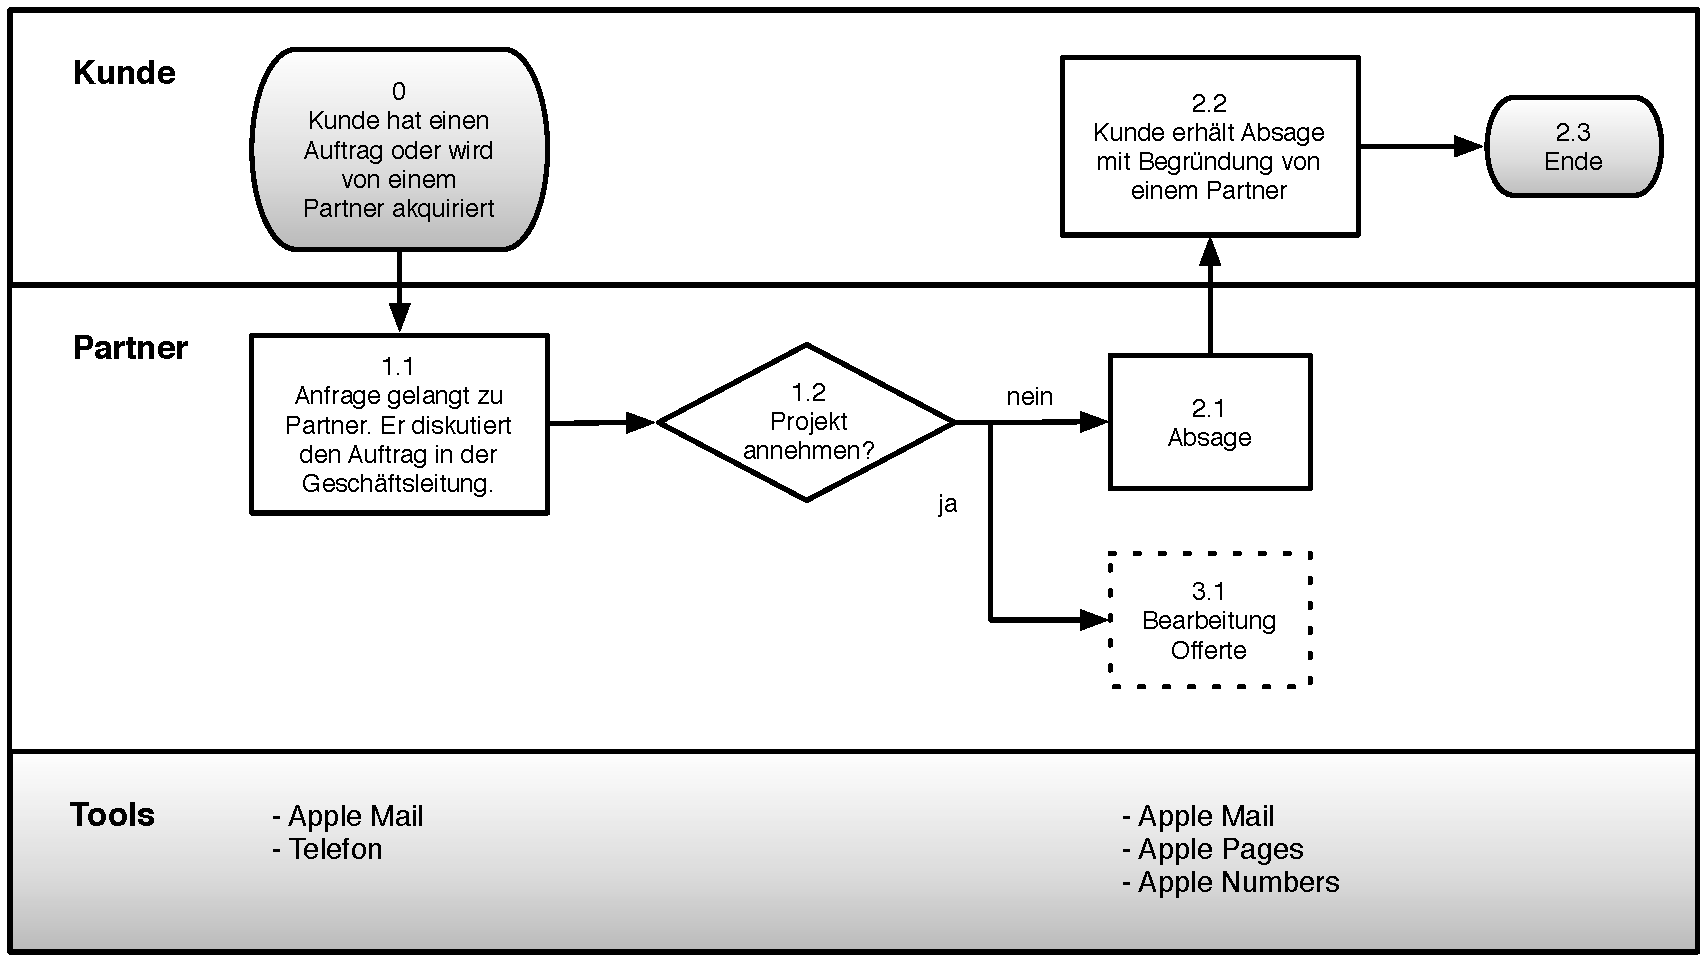
\includegraphics[width=0.99\textwidth,angle=0]{./bilder/analyse/01_ist_prozesse_offerte_01.pdf}
\caption{Offertenerstellungs Prozess von allink März 2011 1/2}
\label{pic:01_ist_prozesse_offerte_01}
\end{center}
\end{figure}

Als Start eines Projektablaufes wird entweder ein neues Projekt akquiriert, 
durch eine direkte Anfrage an ein Unternehmen oder einen Pitch\footnote{Als Pitch 
wird der Wettbewerb zwischen verschiedenen Agenturen um einen Auftrag eines 
Unternehmens bezeichnet.}, oder eine Anfrage kommt direkt von einem Kunden (\textbf{0}). 
Die Projekte gelangen zum heutigen Zeitpunkt immer als erstes zu einem Partner. 
Sehr selten bringt ein Mitarbeiter durch einen seiner Kontakte ein Projekt ein. 
Aber auch in diesem Fall, würde es als erstes an einen Partner herangetragen.
Dieser diskutiert den möglichen Auftrag mit den anderen Partnern in der 
Geschäftsleitung (\textbf{1.1}). Diese entscheide demokratisch ob ein Projekt 
angenommen oder abgelehnt wird (\textbf{1.2}). Sofern nicht alle Partner anwesend 
sein können, haben die anderen Partner die Kompetenz, alleine zu entscheiden.

Im Falle einer Absage (\textbf{2.1}) tritt ein Partner wieder mit dem Kunden in Kontakt.
In den meisten Fällen natürlich der Partner, der bereits mit dem Kunden Kontakt
hatte. Dem Kunden wird erklärt, aus welchen Gründen das Projekt nicht angenommen
und durchgeführt werden kann (\textbf{2.2}).

\begin{figure}[htbp]
\begin{center}
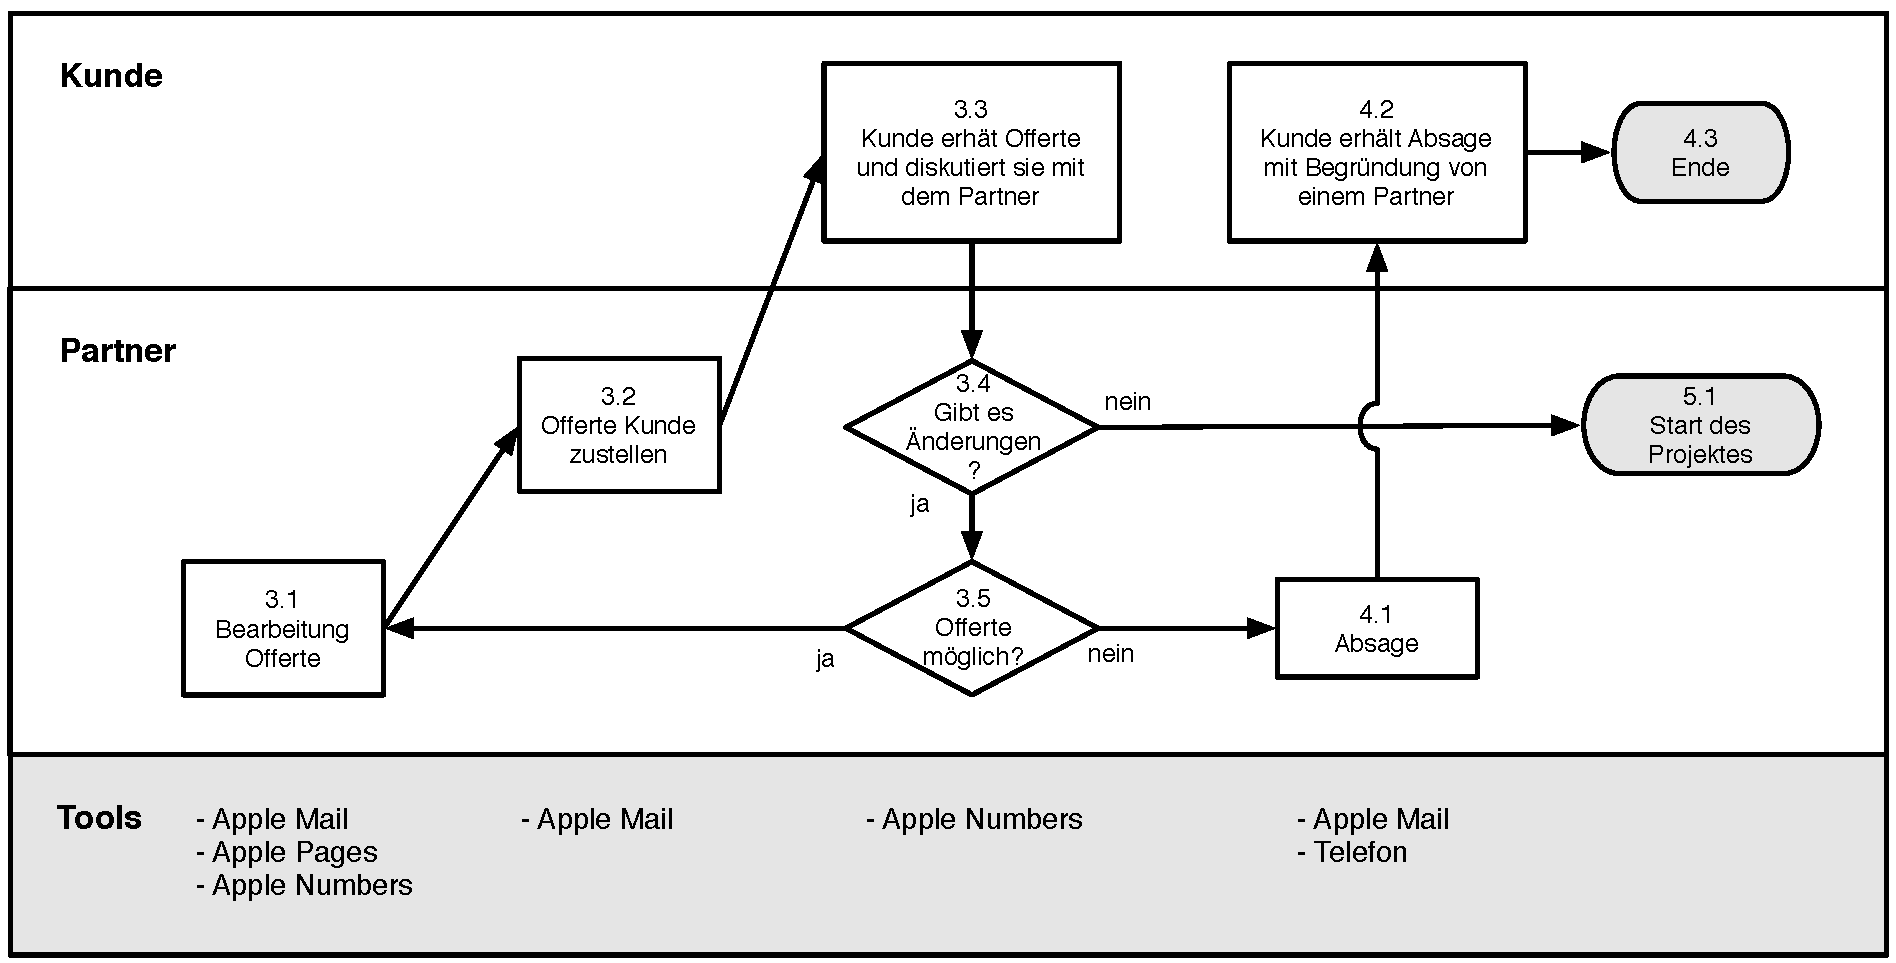
\includegraphics[width=0.99\textwidth,angle=0]{./bilder/analyse/01_ist_prozesse_offerte_02.pdf}
\caption{Offertenerstellungs Prozess von allink März 2011 2/2}
\label{pic:01_ist_prozesse_offerte_02}
\end{center}
\end{figure}

Sollte das Projekt angenommen werden, wird auf Grund den zu erbringenden
Dienstleistungen eine möglichst genaue Offerte erstellt (\textbf{3.1}). Diese Schätzungen
basieren überwiegend auf Erfahrungswerten aus anderen Projekten.
Die Offerte wird dann dem Kunden zugestellt (\textbf{3.2}). In vielen Fällen wird dem Kunden
die Offerte präsentiert und genauer erklärt.
Der Kunde diskutiert dann mit dem oder den Partnern die Offerte (\textbf{3.3}) und bringt
bei bedarf Änderungen und Wünsche an.
Kann man sich mit dem Kunden nicht einigen, also wünscht der Kunde Änderungen
an der Offerte oder den zu erbringenden Dienstleistungen (\textbf{3.4}), die von unserer Seite
nicht mehr möglich sind (\textbf{3.5}), muss das Projekt abgesagt werden (\textbf{4.1}).
Dem Kunden wird erklärt, aus welchen Gründen die Offerte nicht angepasst oder
die Dienstleistung nicht erbracht werden kann (\textbf{4.2}).

Im Falle einer Einigung und einer Auftragserteilung startet das eigentliche
Projekt (\textbf{5.1}).

\clearpage

\subsection{Projektdurchführung}
In der ersten Phase der Projektdurchführung sammelt der Projektleiter bzw.
Partner alle nötigen Informationen, die zur Bearbeitung des Projektes notwendig sind.
Danach erstellt er Arbeitspakete zusammen, die er wiederum an die Mitarbeiter verteilt.
Die Projektdurchführung ist in den Grafiken \ref{pic:02_ist_prozesse_arbeit_01} und 
\ref{pic:02_ist_prozesse_arbeit_02} grafisch dargestellt.

\begin{figure}[htbp]
\begin{center}
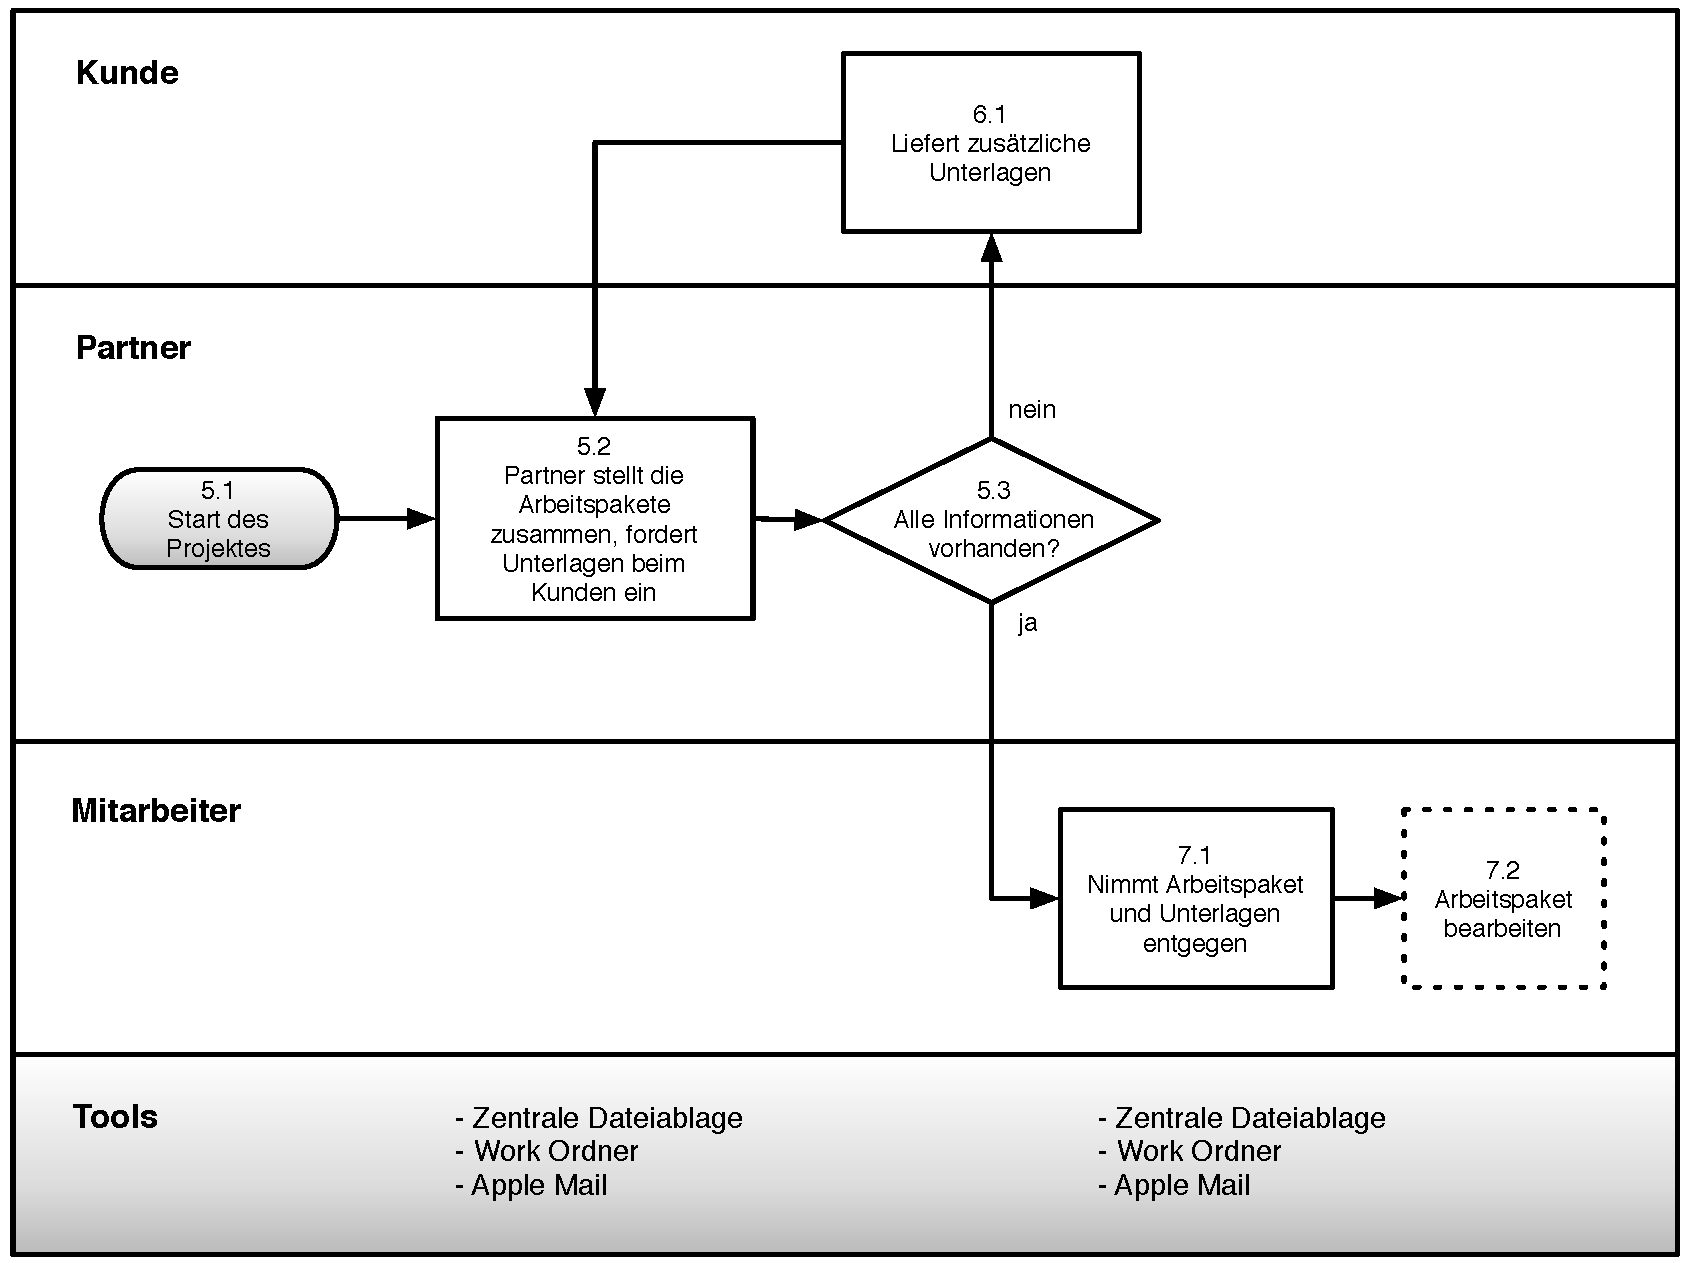
\includegraphics[width=0.99\textwidth,angle=0]{./bilder/analyse/02_ist_prozesse_arbeit_01.pdf}
\caption{Projektumsetzungs Prozess von allink März 2011 1/2}
\label{pic:02_ist_prozesse_arbeit_01}
\end{center}
\end{figure}

Der Partner verschafft sich einen überblick über das Projekt und gruppiert
die zu erledigenden Arbeiten in Arbeitspakete (\textbf{5.2}). Er besorgt alle nötigen Informationen
und Unterlagen, die zur Bewältigung eines Arbeitspaketes notwendig sind und fordert
bei Kunden wenn nötig noch mehr Informationen und Unterlagen ein (\textbf{6.1}).
Sind alle Informationen vorhanden (\textbf{5.3}) übergibt er die Arbeitspakete
den Mitarbeitern zur Erledigung.

Der Mitarbeiter nimmt das Arbeitspaket entgegen (\textbf{7.1}) und beginnt
mit dessen Bearbeitung (\textbf{7.2}). Stellt sich heraus, dass er sein Arbeitspaket
noch nicht abschliessen kann (\textbf{7.3}) und noch mehr Informationen oder
Unterlagen benötigt (\textbf{8.1}), kommt es oft vor, dass der Mitarbeiter
eigenständig beim Kunden zusätzliche Unterlagen einfordert (\textbf{9.1}).
Sobald er ein Paket abschliessen kann, stellt er alles Erarbeitete zusammen (\textbf{10.1})
und übergibt es dem zuständigen Partner bzw. Projektleiter.
Dieser nimmt alle Arbeitspakete entgegen (\textbf{10.2})
und überprüft diese (\textbf{10.3}). Sofern zusätzliche Arbeiten nötig sind,
stellt er diese wieder zusammen und der Bearbeitungsprozess beginnt von neuem (\textbf{5.2}).

\begin{figure}[htbp]
\begin{center}
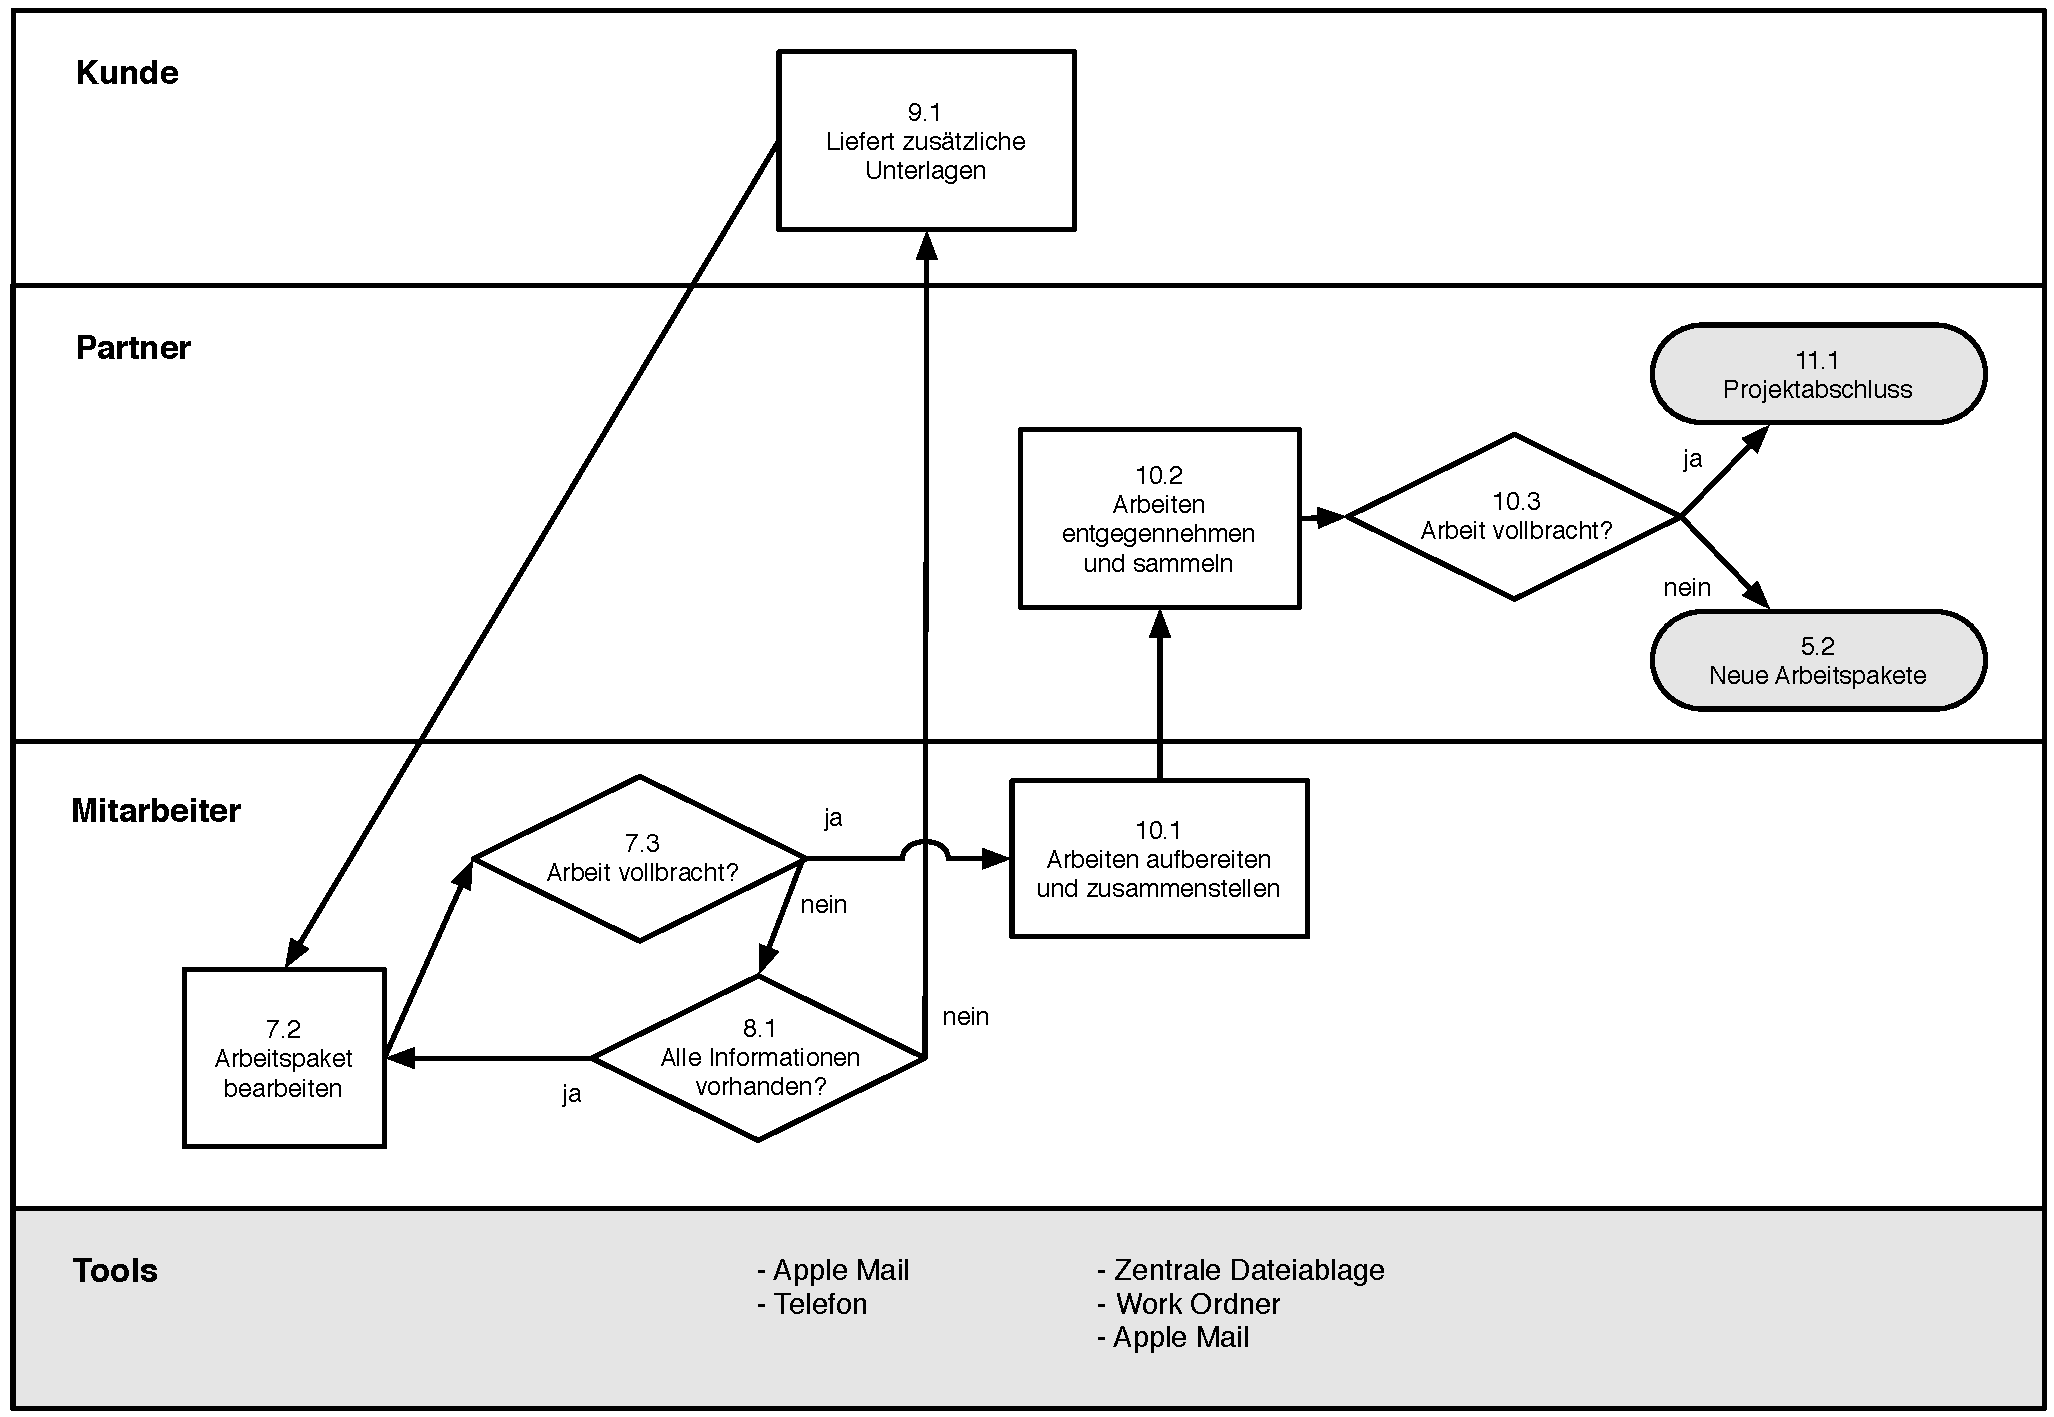
\includegraphics[width=0.99\textwidth,angle=0]{./bilder/analyse/02_ist_prozesse_arbeit_02.pdf}
\caption{Projektumsetzungs Prozess von allink März 2011 2/2}
\label{pic:02_ist_prozesse_arbeit_02}
\end{center}
\end{figure}

Sind alle Arbeiten vollbracht, geht es über in den Projektabschluss (\textbf{11.1}). Dies wirkt
zu früh, da der Kunde bis zu diesem Zeitpunkt noch keine Ergebnisse gesehen
hat. In der Theorie ist die Produktabnahme jedoch auch im Projektabschluss angesiedelt.
Die Präsentation der Resultate und das Feedback des Kunden kommen darin zur Geltung. 
Geht man vom Optimalfall aus, kann das Projekt zu diesem Zeitpunk abgeschlossen 
werden. In der Praxis ist das vor allem bei kleineren Projekten der Fall, wie 
der Erstellung eines neuen Flyers\footnote{Mit einem Flyer bezeichnet man Flugblätter
die zum Transport von Werbebotschaften verwendet werden.}, bei dem sich das Konzept 
über Monate nicht geändert hat und nur Textkorrekturen und leichte visuelle 
Anpassungen notwendig sind. In den meisten Fällen aber kann mit Feedback des
Kunden gerechnet werden, das zu neuen Arbeitspaketen führt.

\subsection{Projektabschluss}
In der nachfolgenden Darstellungen \ref{pic:03_ist_prozesse_abschluss_01} und
\ref{pic:03_ist_prozesse_abschluss_02} ist der aktuelle Prozess des Projektabschlusses 
ersichtlich. Als erstes folgt nun die Präsentation der Arbeit beim Auftraggeber 
bzw. Kunden (\textbf{11.2}). Der Kunde gibt daraufhin Feedback (\textbf{11.3}), 
welches vom Projektleiter entgegengenommen und mit dem Kunden diskutiert wird (\textbf{11.4}).

\begin{figure}[htbp]
\begin{center}
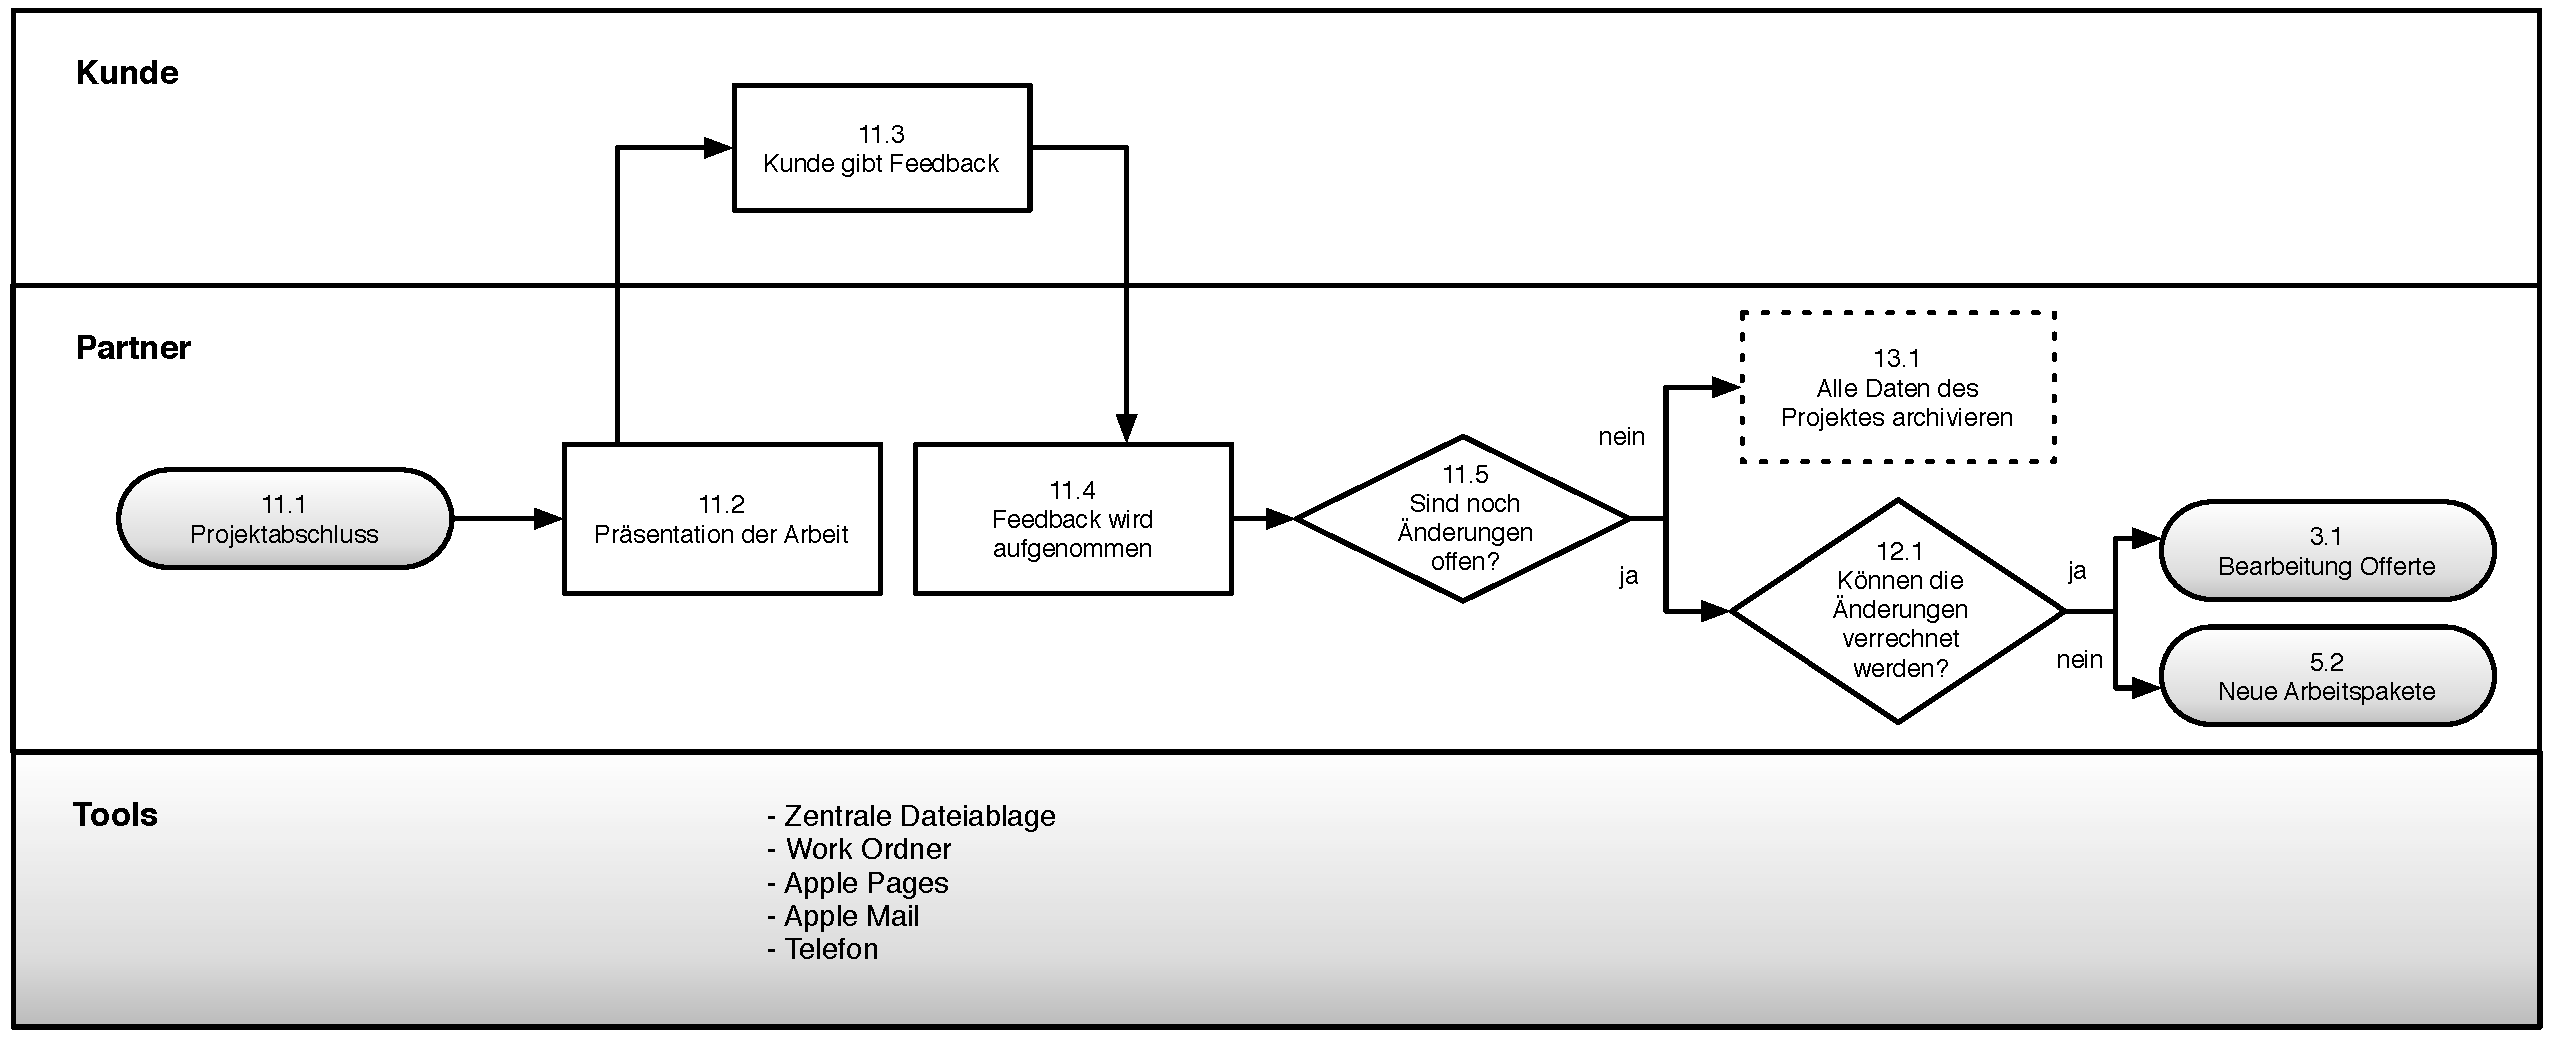
\includegraphics[width=0.99\textwidth,angle=0]{./bilder/analyse/03_ist_prozesse_abschluss_01.pdf}
\caption{Projektabschluss Prozess von allink März 2011 1/2}
\label{pic:03_ist_prozesse_abschluss_01}
\end{center}
\end{figure}

Sofern dann noch Änderungen und Anpassungen nötig sind (\textbf{11.5}), stellt
der Projektleiter bzw. Partner wieder neuen Arbeitspakete zusammen und der
Bearbeitungsprozess beginnt von neuem (\textbf{5.2}). Wenn es sich bei den Wünschen
des Auftraggebers um neue, noch nicht bekannte, Anforderungen handelt, überprüft
der Partner ob eine Anpassung der Offerte notig ist (\textbf{12.1}).

\begin{figure}[htbp]
\begin{center}
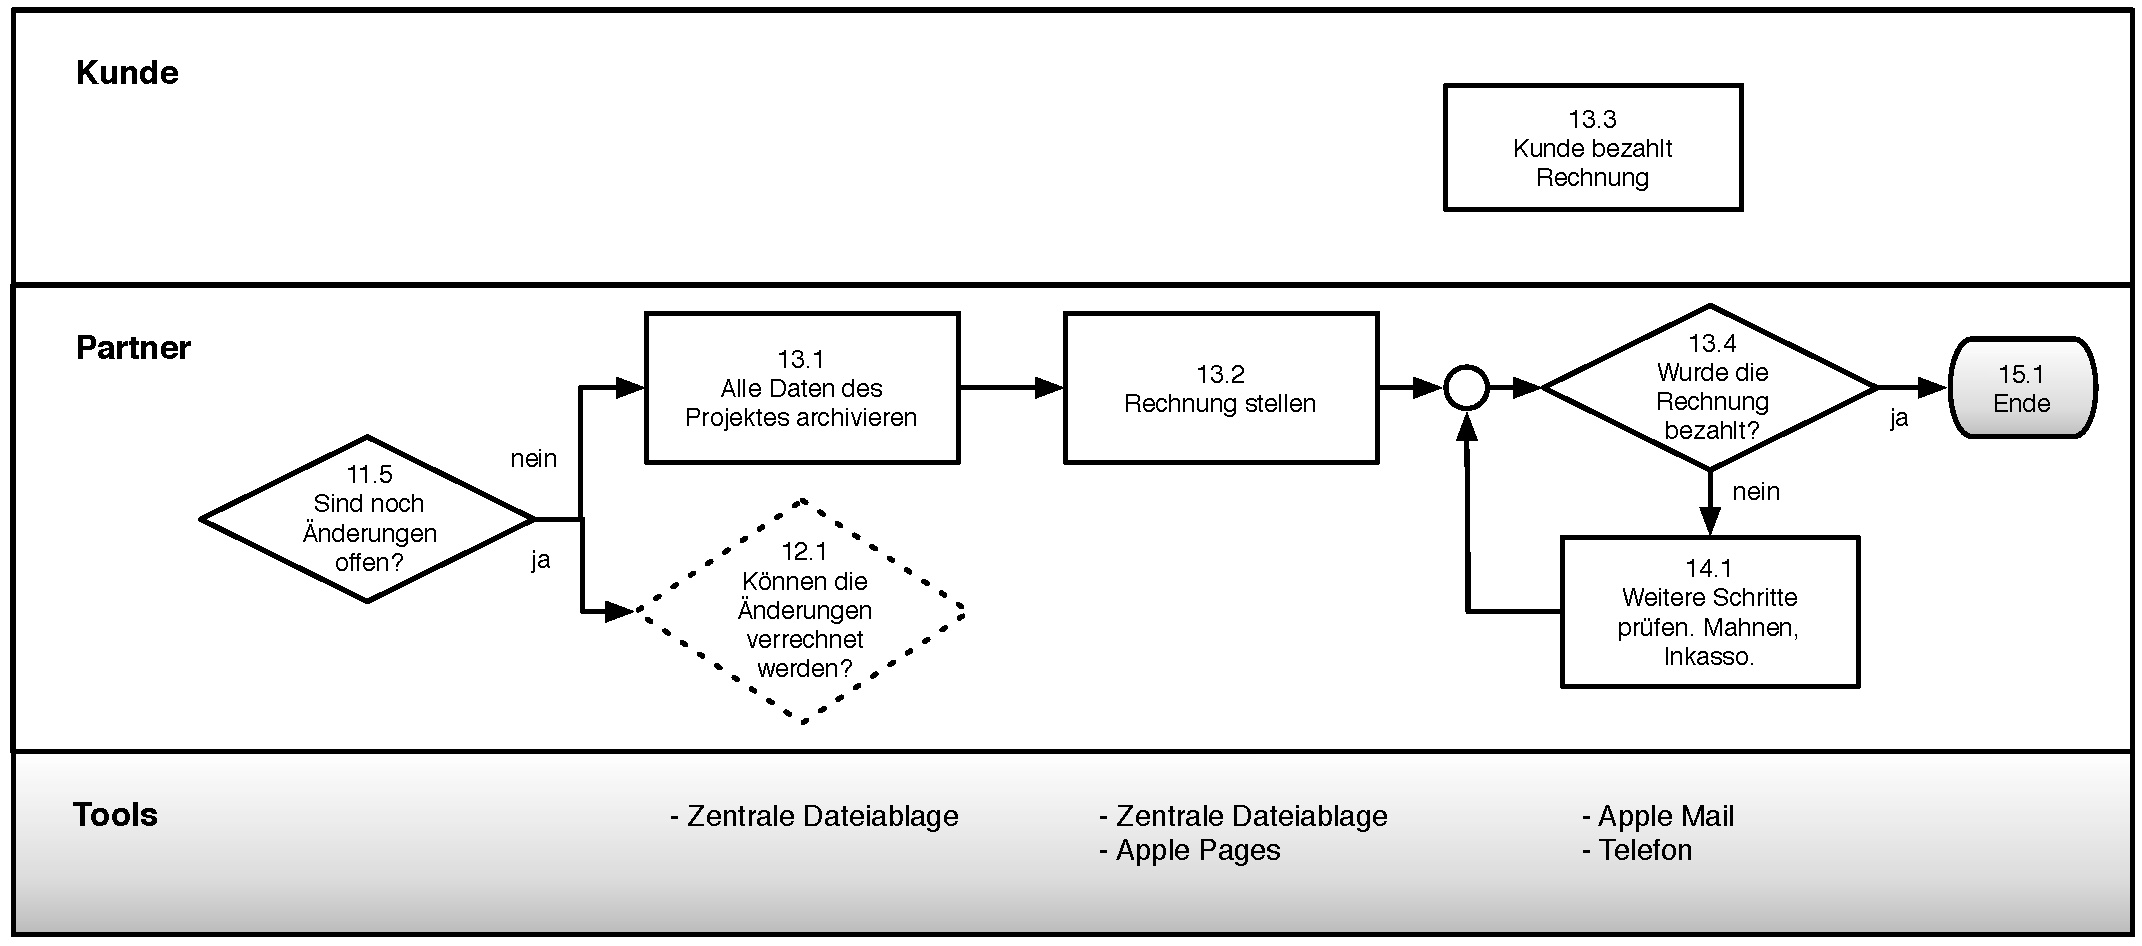
\includegraphics[width=0.99\textwidth,angle=0]{./bilder/analyse/03_ist_prozesse_abschluss_02.pdf}
\caption{Projektabschluss Prozess von allink März 2011 2/2}
\label{pic:03_ist_prozesse_abschluss_02}
\end{center}
\end{figure}

Hier liegt es im Ermessen des Partners, ob es sinnvoll ist die zusätzlichen Kosten 
selbst zu tragen oder in Rechnung zu stellen. Je nach Projektverlauf, auf Grund von
Verzögerungen oder sonstigen Unannehmlichkeiten für den Auftraggeber, kann es
von Nutzen sein dem Kunden zu diesem Zeitpunkt entgegen zu kommen.

Wenn der Auftraggeber zufrieden ist und keine weiteren Anpassungen nötig sind, 
werden alle Daten des Projektes archiviert (\textbf{13.1}). Danach wird die
Endabrechnung durchgeführt und die Abschlussrechnung in Rechnung gestellt (\textbf{13.2}).
Im Verlauf der Zahlungsfrist bezahlt der Kunde die Rechnung (\textbf{13.3}).
Dies wird so lange überwacht (\textbf{13.4}) bis alle offenen Rechnungen beglichen
sind. Wenn eine Rechnung nach der Zahlungsfrist nicht bezahlt wurde, wird
geprüft ob weitere Schritte nötig sind (\textbf{14.1}).

In den meisten Fällen reichen ein paar zusätzliche Tage oder das Nachfragen beim 
Kunden. In den wenigsten Fällen muss gemahnt werden und das Einschalten eines 
Inkassounternehmens war in der Geschichte von allink zum Glück erst ein einziges 
mal notwendig. Sobald alle Rechnungen beglichen sind, gilt das Projekt definitiv 
abgeschlossen (\textbf{15.1}).

\subsection{Verwendete Software}
Bei der Untersuchung der zur Zeit eingesetzten Sofware beschränke ich mich auf jene,
die einen direkten Einfluss auf den aktuellen Projektablauf bei allink haben.
Ich liste keine Software auf, die zur Erbringung der eigentlichen Dienstleistungen
von allink eingesetzt werden.

\begin{figure}[htbp]
\begin{center}
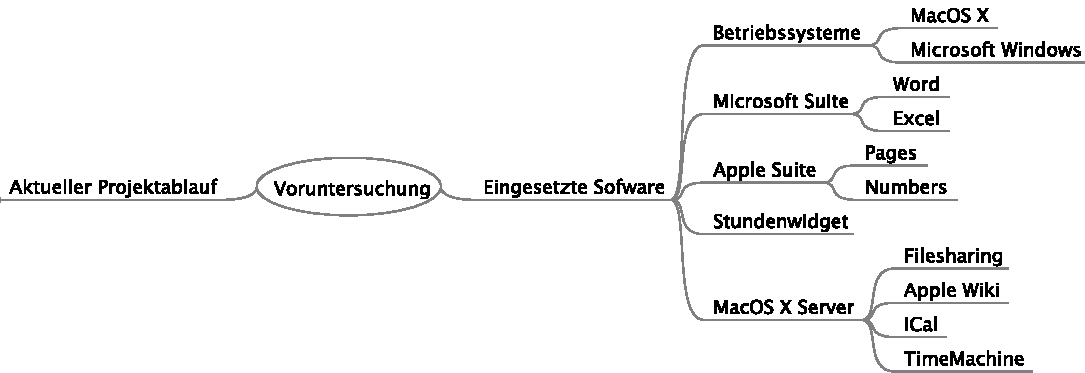
\includegraphics[width=0.95\textwidth,angle=0]{./bilder/analyse/mindmaps/voruntersuchung_software.pdf}
\caption{MindMap Voruntersuchung der eingesetzten Software}
\label{pic:voruntersuchung_software}
\end{center}
\end{figure}

\subsubsection{Betriebssysteme}
Als Hauptbetriebssystem verwendet allink Mac OS X\footnote{Betriebssystem von Apple, \url{http://www.apple.com/macosx/}}.
Es läuft auf allen Arbeitsstationen der Mitarbeiter und Partner. Zusätzlich haben einige der
Entwickler noch Microsoft Windows\footnote{Betriebssystem von Microsof, \url{http://www.microsoft.com/windows/}}
über eine Virtualisierungslösung installiert. Dies wird zu Testzwecken benötigt.

\subsubsection{Microsoft Suite}
Da viele Kunden mit Microsoft Produkten arbeiten benötigt auch allink die
Office Suite\footnote{Microsoft Office für Mac, \url{http://www.microsoft.com/germany/mac}}, 
um Dateien mit Kunden ohne Interoperabilitätsprobleme
austauschen zu können. Nicht jede Arbeitsstation verfügt zur Zeit über eine
Installation.

\subsubsection{Apple Suite}
Für interne Zwecke setzt allink zur Zeit auf die Apple eigene Office Suite
iWork\footnote{Office Suite von Apple, \url{http://www.apple.com/de/iwork/}}.
Pages wird zur Erstellung von Offerten und Rechnungen verwendet. Mit Numbers
werden Tabellenkalkulationen wie die Liquiditätsplanung oder Lohnblätter erstellt.
Da dies aber lange nicht so von der Geschäftsleitung kommuniziert wurde, existieren
auch einige Excel Files, das Pendant der Microsoft Office Suite.

\subsubsection{Stundenwidget}
Das Stundenwidget ist eine selbst geschriebene Software von allink und läuft
im Dashboard\footnote{Widget Lösung von Apple, \url{http://www.apple.com/downloads/dashboard/}} des Betriebssystems.
Es ermöglicht Stunden auf ein Projekt zu buchen, wie man auf dem Screenshot \ref{pic:ist_widget}
sehen kann.

\begin{figure}[htbp]
\begin{center}
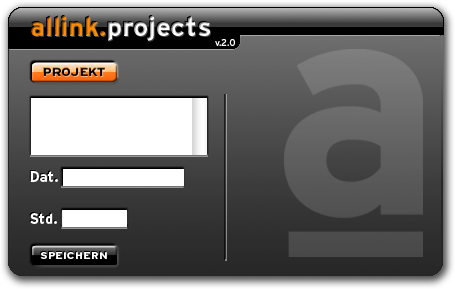
\includegraphics[width=0.55\textwidth,angle=0]{./bilder/analyse/ist_widget.png}
\caption{Aktuelles Stundenwidget von allink}
\label{pic:ist_widget}
\end{center}
\end{figure}

Die Daten werden auf dem
eigenen Server gespeichert und pro Projekt abgelegt. Dieses Widget ist auf allen
Arbeitsstationen installiert und wird von den Mitarbeitern gelegentlich verwendet
um ihre Stunden auf ein Projekt zu rapportieren.

\subsubsection{MacOS X Server}
Auf dem Server liegt das zentrale Dateiablagesystem. Die Zugriffsrechte können
auf dem Server für jede Freigabe definiert werden. So haben zum Beispiel
die Mitarbeiter keinen Zugriff auf den Administrationsordner der Geschäftsleitung.
Über diesen Server laufen auch die einzelnen Firmenkalender der Partner. Sie
können so gemeinsam Termine buchen und haben stets Einblick in die anderen
Kalender.

% \subsection{Methode zur Analyse}
% \subsubsection{Vorgehensmodell nach Grochla}
% Zur Erstellung meiner Ist-Analyse verwende ich die ersten drei Phasen des 
Vorgehensmodell von Erwin Grochla\cite[S. 44-74]{grochla1982grundlagen}.
Die weiteren vier Phasen führen über eine Analyse hinaus und kommen
nicht zur Anwendung.

\subsubsection{Voruntersuchung}
In der Voruntersuchung, auch Pilotstudie genannt, stellt man sich Fragen wie
``Was soll geändert werden?'' und ``Welches sind die Ziele?''. Man verschafft
sich einen Grobüberblick über das eigentliche Problem und die Rahmenbedingungen
möglicher Lösungen. Auch entscheidet man in der Voruntersuchung, ob der Prozess
fortgesetzt oder abgebrochen werden soll. In der Voruntersuchung können die 
meisten Analyse- und Bewertungstechniken verwendet werden.

Nach Absprache mit dem Auftraggeber werde ich mir zur Voruntersuchung mit  
Hilfe von MindMaps einen besseren Überblick über die aktuellen Probleme bei
allink verschaffen. Auf die einzelnen Punkte soll genauer eingegangen
und wenn möglich Fallbeispiele aus der Praxis genannt werden.

Ich verwende die Technik der MindMaps schon seit einigen Jahren und verwende
sie sehr oft in Projekten um mir einen Überblick über Themen zu verschaffen.

\begin{quote}
Eine Mind-Map beschreibt eine besonders von Tony Buzan geprägte kognitive 
Technik, die z.B. zur Erschliessung und visuellen Darstellung eines Themengebietes, 
zur Planung oder für Mitschriften genutzt werden kann. Hierbei soll das Prinzip 
der Assoziation helfen, Gedanken frei zu entfalten und die Fähigkeiten des Gehirns 
zu nutzen. Die Mind-Map wird nach bestimmten Regeln erstellt und gelesen. Den 
Prozess bzw. das Themengebiet bzw. die Technik bezeichnet man als Mind-Mapping.
\cite{wikipedia_mindmap}
\end{quote}

\subsubsection{Ist-Aufnahme}
In der zweiten Phase erfasst man den aktuellen Zustand indem man das zu 
Untersuchende aus möglichst vielen Betrachtungswinkeln analysieren. Zu den
Techniken der Ist-Aufnahme zählen die Selbstaufschreibung, die Befragung und 
die Beobachtung.

Ich werde mit mir selbst eine Selbstaufschreibung durchführen, da ich in meinem 
Arbeitsalltag unseren Problemen genau so ausgesetzt bin. Aber da mir nur begrenzt
Zeit zur Verfügung steht und damit die Mitarbeiter möglichst ungestört arbeiten
können, begrenze ich Befragungen auf die Partner. Die Meinungen und Beobachtungen
aller Partner fliesst dann in die Ist-Aufnahme ein.

\subsubsection{Ist-Kritik}
In der dritten Phase widmet man sich den erhobenen Informationen aus der zweiten Phase. 
Die genauen Ursachen der Probleme sollen herausgeschält werden, damit nicht nur 
Symptome behandelt werden. 

Um die Probleme auf ihre tatsächlichen Ursachen zurückführen zu können,
werde ich eine Form der Prüfmatrix, eine Problem-Ursachen Matrix, erstellen.

\begin{quote}
    Die Prüfmatrix ist ein vereinfachtes Verfahren um Mängel und deren Ursachen 
    zu ermitteln. Mängel werden dabei möglichen Ursachenkategorien matrixförmig 
    gegenübergestellt. Im Schnittpunkt von Mangel und Ursachenkategorie werden 
    die tatsächlichen Ursachen gesucht.\cite{schmidt2000methode}
\end{quote}

\subsection{Stärken und Schwächen}
In diesem Kapitel werden die Stärken und Schwächen des aktuellen Projektablaufes
der allink und der darin verwendeten Software genauer untersucht. Als Methode
eignet sich dazu eine SWOT-Analyse. Die SWOT-Analyse ist ein Instrument um
Stärken, Schwächen, Chancen und Risiken darzustellen. Es eignet sich sowohl zur Situationsanalyse
wie auch als Instrument der Strategieformulierung.\footnote{\citealp*[Vgl.][S. 134]{homburg2000quantitative}}
In der folgenden Grafik \ref{pic:swot_analyse} ist die SWOT-Analyse des Projektablaufes
von allink abgebildet.

\begin{figure}[htbp]
\begin{center}
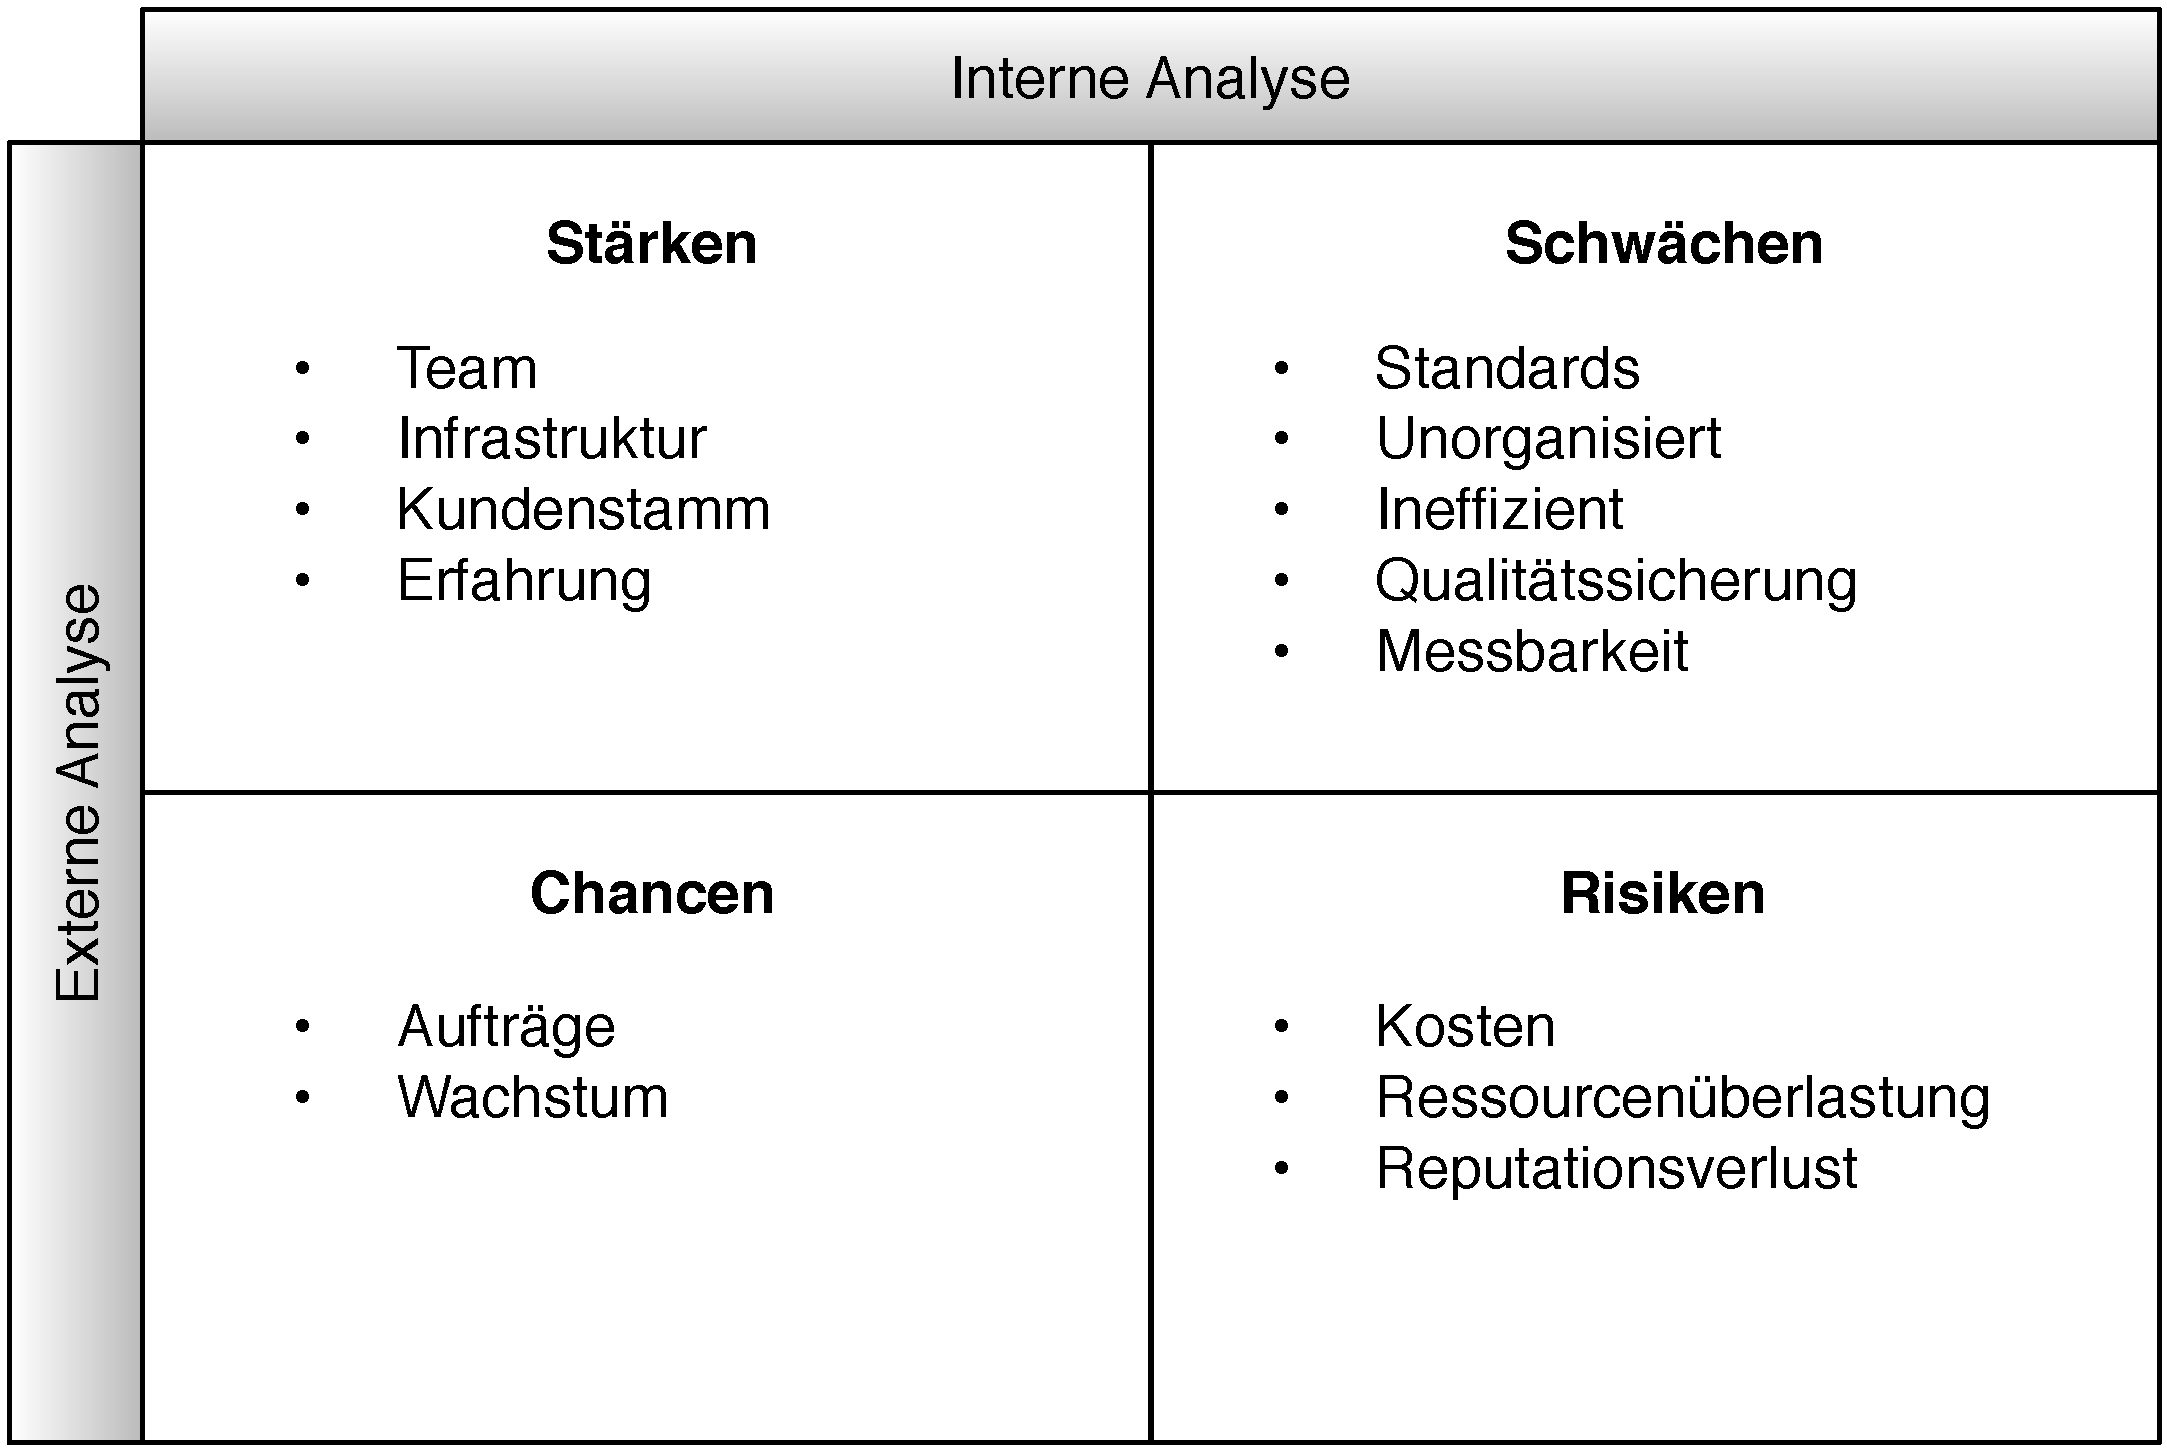
\includegraphics[width=0.8\textwidth,angle=0]{./bilder/analyse/swot_analyse.pdf}
\caption{SWOT-Analyse des Projektablaufes von allink}
\label{pic:swot_analyse}
\end{center}
\end{figure}

Es wird nun im Detail auf die einzelnen Punkte aus der SWOT-Analyse eingegangen
und wo möglich mit einem Beispiel aus der Praxis untermalt.

% Die Ressourcenüberbelastung ist nur ein Problem, das zum Vorschein kommt. In der
% Abbildung \ref{pic:voruntersuchung_projektablauf} verschaffe ich mir einen 
% Überblick über die möglichen Gefahren und Schwächen des aktuellen Projektablaufes.
% 
% \begin{figure}[htbp]
% \begin{center}
% 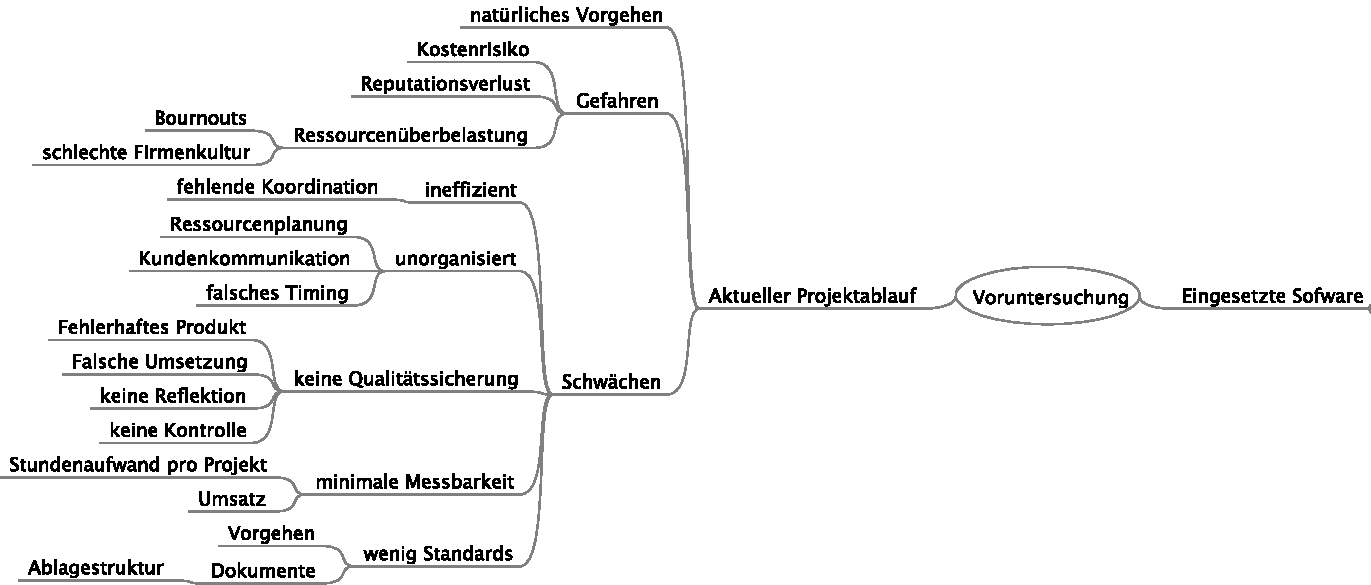
\includegraphics[width=0.95\textwidth,angle=0]{./bilder/analyse/mindmaps/voruntersuchung_projektablauf.pdf}
% \caption{MindMap Voruntersuchung des aktuellen Projektablaufes}
% \label{pic:voruntersuchung_projektablauf}
% \end{center}
% \end{figure}

\subsubsection{Wenig Standards}
Man hält vor, während und nach einem Projekt nur an wenige Standards fest. 
Das ganze Vorgehen ist nicht einheitlich, da in jedem Projekt wieder von
neuem entschieden wird, wie man vorgehen will. Es werden nur wenige einheitlichen
Dokumente verwendet, zum Beispiel für die Erstellung von Offerten und Rechnungen.
Aber auch da entstehen schnell Fehler, z.B. während der Umstellungen des 
Mehrwert Steuersatzes von 7.6\% auf 8\%. Da kein einheitliches Basistemplate
existiert, muss jeder der eine Rechnung schreibt noch einmal sicherstellen, ob
auch der korrekte Steuersatz hinterlegt ist. 

\subsubsection{Unorganisiert}
Durch die Überbelastung können mit der Zeit die versprochenen Timings
nicht mehr eingehalten werden. Da die Ablagestrukturen nicht einheitlich geregelt
sind, kann es vorkommen, dass ein Mitarbeiter einem Kunden ein veraltetes oder
noch nicht freigegebenes Dokument sendet. Dies zieht einen zusätzlichen 
Mehraufwand mit sich, da man sich beim Kunden entschuldigen und rechtfertigen
muss. Zusätzlich strapaziert es auch die Beziehung zum Kunden.

\subsubsection{Ineffizient}
Einfache Abläufe werden so unnötig verkompliziert und aufgehalten. Die ganze
Struktur wird langsam und ineffizient. Was sich wiederum negativ auf die zur
Verfügung stehende Zeit auswirkt.

\subsubsection{Keine Qualitätssicherung}
Oft bleibt gegen Ende eines Projektes dann zu wenig Zeit die nötige 
Qualitätskontrollen durchzuführen, da man sich möglichst schnell um ein anderes,
möglicherweise auch schon überfälliges, Projekt kümmern muss. Der Kunde entdeckt
dann offensichtliche Fehler selbst und zweifelt zwangsläufig an der ganzen Arbeit.

\subsubsection{Minimale Messbarkeit}
Auch bietet die fehlende bzw. chaotische Struktur nur wenige Punkte um Kennzahlen
zu messen. Den Umsatz den man mit dem Projekt erzielt hat ist zwar bekannt,
jedoch kann nur aus dem Gefühl heraus erahnt werden, ob mit dem Projekt einen
Gewinn für die Firma erzielt werden konnte. Die Mitarbeiter sind zwar angehalten
ihre Stunden in ein gemeinsames Stundelog pro Projekt einzutragen, jedoch werden
die Informationen nicht ausgewertet und können nicht mehr einzelnen Mitarbeitern
zugeordnet werden.

\subsubsection{Kostenrisiko}
Durch die fehlende Kontrolle während eines Projektes, verliert man die
Übersicht über die Aufwände und schlussendlich die Kosten. Dadurch entsteht
ein Kostenrisiko, welches Konsequenzen für die Liquidität von allink haben könnte.

\subsubsection{Ressourcenüberbelastung}
Die Belastung für den Mitarbeiter wie auch für die Partner ist so über
längere Zeit nicht tragbar. Durch eine Überarbeitung kann es zu Ausfällen kommen, die
die Situation zusätzlich verschlimmern könnten. Das ganze Endet in einer 
schlechten Firmenkultur und das Unternehmung beginnt von innen zu zerfallen.

\subsubsection{Reputationsverlust}
Da man Timings nicht mehr einhalten kann und man sich gegenüber dem Kunden
oft rechtfertigen muss entsteht ein schlechtes Bild der Unternehmung und sie
verliert an Vertrauen. Da die Konkurrenz im Tätigkeitsfeld der allink relativ
gross ist, ist ein möglicher Absprung und Angenturwechsel seitens des Kunden nicht 
auszuschliessen.


\section{Marktanalyse}
\subsection{Panter IIc}

\section{Konklusion}
